\documentclass[sigconf,review,anonymous]{acmart}

\usepackage{amsmath}
\usepackage{booktabs}
\usepackage{graphicx}
\usepackage{xcolor}
\usepackage{algorithm}
\usepackage{algorithmic}
\usepackage{pifont}
\usepackage{subcaption}
\usepackage{multirow}
\usepackage{enumitem}
\setlength{\emergencystretch}{3em}
% Submission-page economy: tighten float and list spacing without changing the ACM format.
\setlength{\textfloatsep}{6pt plus 2pt minus 2pt}
\setlength{\floatsep}{6pt plus 2pt minus 2pt}
\setlength{\intextsep}{6pt plus 2pt minus 2pt}
% Tighten only user-facing lists; avoid changing description or package-internal lists.
\setlist[itemize]{nosep,leftmargin=*}
\setlist[enumerate]{nosep,leftmargin=*}

\graphicspath{{./}{figures/}{../figures/}}

% Remove ACM copyright for draft
\setcopyright{none}
\settopmatter{printacmref=false}
\makeatletter
\@ifundefined{footnotetextcopyrightpermission}{}{%
  \renewcommand\footnotetextcopyrightpermission[1]{}%
}
\makeatother

% Anonymous review metadata for ACM submission.
\acmConference[Anonymous Submission]{Anonymous Submission}{2026}{Anonymous}
\acmYear{2026}
\copyrightyear{2026}
\acmISBN{}
\acmDOI{}


\begin{document}

\title{PlanGate: Session Commitment for Multi-Step LLM Agent Tool Governance}

\author{Anonymous}
\affiliation{\institution{Anonymous Institution}\country{}}
\email{anonymous@example.com}

% ABSTRACT
\begin{abstract}
Multi-step LLM agents expose a governance mismatch that request-oriented overload control does not directly address: the \emph{governance unit} is an individual tool call, while the \emph{workload unit} is a dependent multi-step session. A rejection at step~$K$ therefore wastes the compute invested in steps~$1$--$K{-}1$. We propose \emph{session commitment}---atomic admission, temporal isolation, and continuation value---and implement it in \textsc{PlanGate}, an MCP-compatible gateway. PlanGate combines budget-reserved commitments for declared Plan-and-Solve sessions, sunk-cost-aware continuation pricing for ReAct sessions, commitment tokens for client-visible admission integrity, bounded plan amendment for recoverable plan drift, checkpoint-aware recovery, and optional Redis-backed shared state. The evidence is deliberately scoped. In controlled mock workloads, PlanGate converts mid-session failures into zero-compute-waste step-0 rejections, reaching 54.8 effective GP/s with 0.2 cascade failures per run in the refreshed core experiment. Under failure/amendment workloads, the full mechanism completes 192.3 of 200 sessions on average, while disabling commitment, amendment, or recovery degrades success and disables the corresponding signal. In two-gateway CloudLab validation, Redis-backed checkpoint/reservation state records 843 cross-node sessions with zero state misses or duplicate admissions. Real-LLM GLM and DeepSeek runs are treated as smoke/support evidence rather than dominance claims: they confirm provider compatibility and show the same boundary behavior under elastic commercial APIs. Session commitment's value is therefore strongest under hard or bursty resource constraints, while its cost is conservative admission when backend headroom is abundant.
\end{abstract}

\maketitle

% 1. INTRODUCTION
\section{Introduction}

Modern LLM agents decompose complex tasks into sequences of tool calls. Plan-and-Solve (P\&S)-style agents~\cite{planandsolve} can expose an upfront plan, which PlanGate represents as a DAG for admission control, while ReAct agents~\cite{react} interleave reasoning and acting and reveal actions incrementally. Both patterns create \emph{multi-step sessions}: ordered chains of 3--10 tool invocations where each step depends on previous results. The Model Context Protocol (MCP)~\cite{mcp2024} standardizes these interactions via JSON-RPC, enabling interoperable tool ecosystems. Building on chain-of-thought reasoning~\cite{cot}, modern agent frameworks extend LLMs from passive responders to active tool-using agents~\cite{llmsurvey}. As agentic systems scale to hundreds of concurrent users, the tool-serving infrastructure must govern access to shared resources---but governance must respect \emph{session semantics}: a session has value only if all its steps complete; partial execution produces no useful result. While PlanGate is designed and tested on MCP, its session commitment abstraction applies to any multi-step tool-calling protocol; MCP serves as the deployment surface, not the theoretical foundation. In this sense, PlanGate acts as a governance layer for MCP-style agent tool-serving systems.


Existing overload control governs at the wrong granularity. Static rate limiting treats each tool call independently; microservice admission control systems such as DAGOR~\cite{dagor} and Breakwater~\cite{breakwater} shed requests based on instantaneous load; even Rajomon~\cite{rajomon2025} (NSDI'25), which adapts prices via queuing delay, prices individual RPCs without distinguishing a session's first call from its tenth. All these systems share a fundamental flaw: their \emph{governance unit is the individual request}, while the \emph{workload unit is the multi-step session}. This mismatch causes \emph{cascading compute waste}---when a session is admitted at step~0 but rejected at step~$K$, the compute invested in steps~$1$--$K{-}1$ is irrecoverably lost. Under 200-concurrent-session load with no governance, 65\% of admitted sessions are doomed to fail mid-execution.

Session commitment is not a new algorithmic primitive; it is a new \emph{systems abstraction}. The individual mechanisms---admission control, price locking, and convex discounting---are well understood in isolation. Our contribution is demonstrating that their \emph{composition under session-level semantics} addresses a structural waste pattern that per-request governance is fundamentally ill-equipped to avoid, because its governance unit does not match the workload unit.


This waste is not merely a tuning issue but reflects a systematic mismatch. We demonstrate through a sensitivity scan over Rajomon's \texttt{price\_step} parameter ($\{5, 10, 20, 50, 100\}$, 5 repeats each) that per-request pricing struggles to provide session-level protection across its parameter range. The best-case configuration (\texttt{price\_step=5}) achieves an admitted-but-doomed rate (ABD) of 64.4\%---comparable to no governance (65.5\%)---because the pricing signal is too weak to reject overload, providing minimal session-level differentiation. At higher price steps (${\geq}20$), ABD rises above 89\% as aggressive per-request pricing ejects mid-session requests more frequently. Neither extreme provides session protection; per-request governance systematically fails to account for the sequential dependencies within sessions.


We identify three properties that a governance system must provide to support multi-step agent workloads:
\begin{enumerate}[nosep,leftmargin=*]
  \item \emph{Atomic admission}: the system evaluates the session's full resource needs at step zero, ensuring that partial execution never begins unless the system can sustain the full session.
  \item \emph{Temporal isolation}: once admitted, a session's pricing is locked for its lifetime, shielding it from price increases caused by subsequently arriving sessions.
  \item \emph{Continuation value}: the effective admission cost decreases as a session progresses, reflecting the growing sunk cost~\cite{sunkcost_econ} and the increasing waste of rejection.
\end{enumerate}
We call the conjunction of these properties a \emph{session commitment}. Crucially, the two dominant agent types receive \emph{different strengths of commitment}: P\&S agents that declare full plans receive \emph{budget-reserved} commitments---scoped price-isolation protection against price-induced mid-session rejection, contingent on reservation validity, backend availability, and plan accuracy. ReAct agents, which cannot declare plans upfront, receive \emph{soft} commitments---sunk-cost-aware continuation incentives that substantially reduce, but cannot eliminate, mid-execution abandonment. This distinction is fundamental and intentional, not a limitation: the two agent types expose different information at admission time and therefore warrant different commitment semantics.


We implement session commitment in \textsc{PlanGate}, a plan-aware MCP-compatible gateway deployed as a transparent reverse proxy between LLM agent clients and MCP-compatible tool servers. For P\&S agents, PlanGate performs pre-flight atomic admission over the declared DAG plan and, upon admission, creates a budget reservation that locks prices for the session's lifetime---within the declared plan scope, under valid reservations, available backends, and plan-accurate execution, this shields admitted sessions from price-induced mid-session rejection (ABD\textsubscript{P\&S}$\,{=}\,$0.0\% only in controlled mock experiments). For ReAct agents, PlanGate applies sunk-cost-aware dynamic pricing with a quadratic discount $1/(1{+}K^2\alpha)$ at step~$K$, providing a soft commitment that reduces ABD\textsubscript{ReAct} from 54--65\% (baselines) to 21.7\%. Both modes are unified under a single gateway using header-driven routing and a governance intensity signal that adapts admission to real-time backend load.

PlanGate makes three contributions:

\noindent\textbf{(1) Problem abstraction: session-level governance.} We identify cascading compute waste as a structural mismatch between request-level governance and session-level workload semantics. We formalize \emph{session commitment} as the conjunction of atomic admission, temporal isolation, and continuation value, and use admitted-but-doomed rate (ABD), stratified by agent mode, as a system-semantic metric for commitment quality.

\noindent\textbf{(2) PlanGate design and implementation.} We design and implement an MCP-compatible gateway that provides budget-reserved, scoped price-isolation protection for plan-accurate P\&S agents and sunk-cost-aware soft commitments for ReAct agents. The implementation combines pre-flight DAG admission, locked-price budget reservation, continuation-aware pricing, load-sensitive governance intensity, commitment tokens, bounded amendment, checkpoint-aware recovery, and optional Redis-backed shared state in a single reverse proxy.

\noindent\textbf{(3) Evidence hierarchy and boundary characterization.} Across controlled mock experiments, failure/amendment ablations, CloudLab shared-state validation, and provider-backed smoke runs, we compare PlanGate against request-level and session-level baselines. The results show that session commitment substantially reduces ABD and cascading waste under hard or bursty constraints, while real-LLM smoke runs delineate the elastic-provider boundary rather than establishing universal dominance. A throughput--latency summary over Exp1/Exp5/Exp6/Exp10 consolidates raw/effective goodput and P95 latency, and a two-gateway validation demonstrates the deployment boundary: without shared state, random per-step routing creates continuation state misses; with Redis-backed state, those misses drop to zero despite real cross-node execution.

\section{Background and Motivation}


\subsection{MCP and Multi-Step Tool Calling}

The Model Context Protocol (MCP) standardizes how LLM agents discover and invoke external tools via JSON-RPC 2.0. A client sends a \texttt{tools/call} request containing the tool name, input arguments, and optional metadata (\texttt{\_meta}); the server executes the tool and returns structured results. MCP itself specifies tool invocation rather than session-level overload semantics; in agent workloads built over MCP, a single user task often forms a session of 3--10 sequential tool calls, each building on previous results.


Modern LLM agents employ two dominant reasoning strategies. \emph{Plan-and-Solve}-style (P\&S) agents can expose an upfront plan, which PlanGate represents as a DAG of tool calls with dependencies for admission control. \emph{ReAct} agents interleave reasoning and acting: they decide the next tool call based on the observation from the previous step, without a predetermined plan. Both patterns create multi-step sessions where mid-execution failures cause cascading waste, but they differ fundamentally in how much information is available for admission control: P\&S agents can declare their full resource needs upfront, while ReAct agents cannot.


\subsection{The Cascading Compute Waste Problem}

Consider a ReAct agent executing a 5-step task under overload. Suppose the first three tool calls succeed, each consuming 1 second of compute and LLM inference tokens. If the fourth call is rejected by a stateless rate limiter, the 3 seconds of compute and all associated LLM tokens are wasted---the partial results cannot be used, and the user receives a failure. We define this as \emph{cascading compute waste}: the retroactive invalidation of successfully completed work due to a downstream admission failure.


This problem is structurally absent from traditional microservice workloads, where each request is independent. In agentic workloads, however, requests within a session form a \emph{sequential dependency chain}: step $k+1$ cannot begin until step $k$ completes, and the value of step $k$ is zero unless all subsequent steps also complete. This creates an asymmetry that existing admission control ignores: the cost of rejecting a request at step $k$ grows with $k$, as more prior compute is wasted.

\textbf{Terminology.} We distinguish four related concepts used throughout this paper: (1)~a \emph{cascade failure} is the event where an admitted session is rejected at step $K>0$, invalidating prior work; (2)~\emph{cascading waste} is the total wasted compute (tokens, tool calls, wall-clock time) caused by cascade failures; (3)~a \emph{doomed session} (reported as PARTIAL in our metrics) is a session that passes step-0 admission but ultimately fails mid-execution---the session-level unit of cascade failures; (4)~a \emph{step-0 rejection} blocks a session before tool execution begins, incurring zero compute waste but still affecting user-facing availability. The \emph{admitted-but-doomed rate} (ABD) is the fraction of admitted sessions that become doomed.


\subsection{Limitations of Existing Approaches}

\begin{table}[t]
\caption{Comparison of overload control approaches for multi-step workloads. \emph{Session Aware} = tracks cross-request state; \emph{Atomic Admit} = whole-plan admission; \emph{Temporal Isol.} = admitted sessions shielded from price volatility; \emph{Continuation Val.} = progress-dependent effective cost reduction.}
\label{tab:comparison}
\small
\resizebox{\columnwidth}{!}{%
\begin{tabular}{@{}lccccc@{}}
\toprule
\textbf{System} & \textbf{Session} & \textbf{Atomic} & \textbf{Temporal} & \textbf{Continuation} & \textbf{Scoped} \\
 & \textbf{Aware} & \textbf{Admit} & \textbf{Isol.} & \textbf{Val.} & \textbf{Cascade}$^*$ \\
\midrule
SRL & \ding{55} & \ding{55} & \ding{55} & \ding{55} & \ding{55} \\
Breakwater & \ding{55} & \ding{55} & \ding{55} & \ding{55} & \ding{55} \\
SBAC & \checkmark & \ding{55} & \ding{55} & \ding{55} & \ding{55} \\
Rajomon & \ding{55}$^\dagger$ & \ding{55} & \ding{55} & \ding{55} & \ding{55} \\
\textbf{PlanGate} & \checkmark & \checkmark & \checkmark & \checkmark & \checkmark \\
\bottomrule
\end{tabular}}
\vspace{-0.3em}
{\footnotesize $^\dagger$Rajomon prices individual RPCs; it has no session-level state.\\
$^*$Scoped cascade protection means price-induced cascade protection within declared P\&S plan scope under controlled mock (Tier\,1) conditions, valid reservations, available backends, and plan-accurate execution; for real-LLM results see \S\ref{sec:bursty_reallm}.}
\end{table}

Table~\ref{tab:comparison} summarizes how existing systems handle multi-step workloads. SRL, DAGOR, and Breakwater treat each request independently---they are session-oblivious. SBAC limits concurrent sessions but provides no economic pricing or sunk-cost awareness. Rajomon adapts prices via queuing delay but its per-request model means a session at step~8 faces the same price as at step~1, despite $8\times$ more invested compute at risk. None of these systems provide \emph{session commitment}: (a)~atomic admission, (b)~temporal isolation, or (c)~continuation value. To the best of our knowledge, PlanGate is the first MCP-compatible governance design that jointly implements atomic admission, temporal isolation, and continuation value under a session-commitment abstraction.


% 3. SYSTEM DESIGN
\section{System Design}

\subsection{Architecture Overview}

PlanGate is implemented as a Go-based HTTP reverse proxy that sits between LLM agent clients and a Python MCP-compatible backend server. Figure~\ref{fig:arch} illustrates the three-tier architecture. Agent clients send standard MCP JSON-RPC 2.0 requests augmented with governance headers (\texttt{X-Plan-DAG}, \texttt{X-Session-ID}, \texttt{X-Total-Budget}, commitment-token metadata, and optional recovery/amendment metadata). The PlanGate gateway intercepts every \texttt{tools/call} request, makes an admission decision, and either forwards the request to the backend or returns a JSON-RPC error with code \texttt{-32001} (overloaded). The gateway maintains five stateful components: (1) a queuing-delay-based dynamic price table, (2) a session budget reservation manager for P\&S sessions, (3) a ReAct session tracker for sunk-cost-aware pricing, (4) commitment-token and amendment bookkeeping, and (5) a checkpoint store that can be in-memory or Redis-backed. Although the current implementation uses MCP's JSON-RPC transport, the governance logic operates on protocol-independent metadata (session ID, step count, budget declaration); adapting to other multi-step tool-calling protocols requires only a thin transport adapter.


\begin{figure*}[t]
\centering
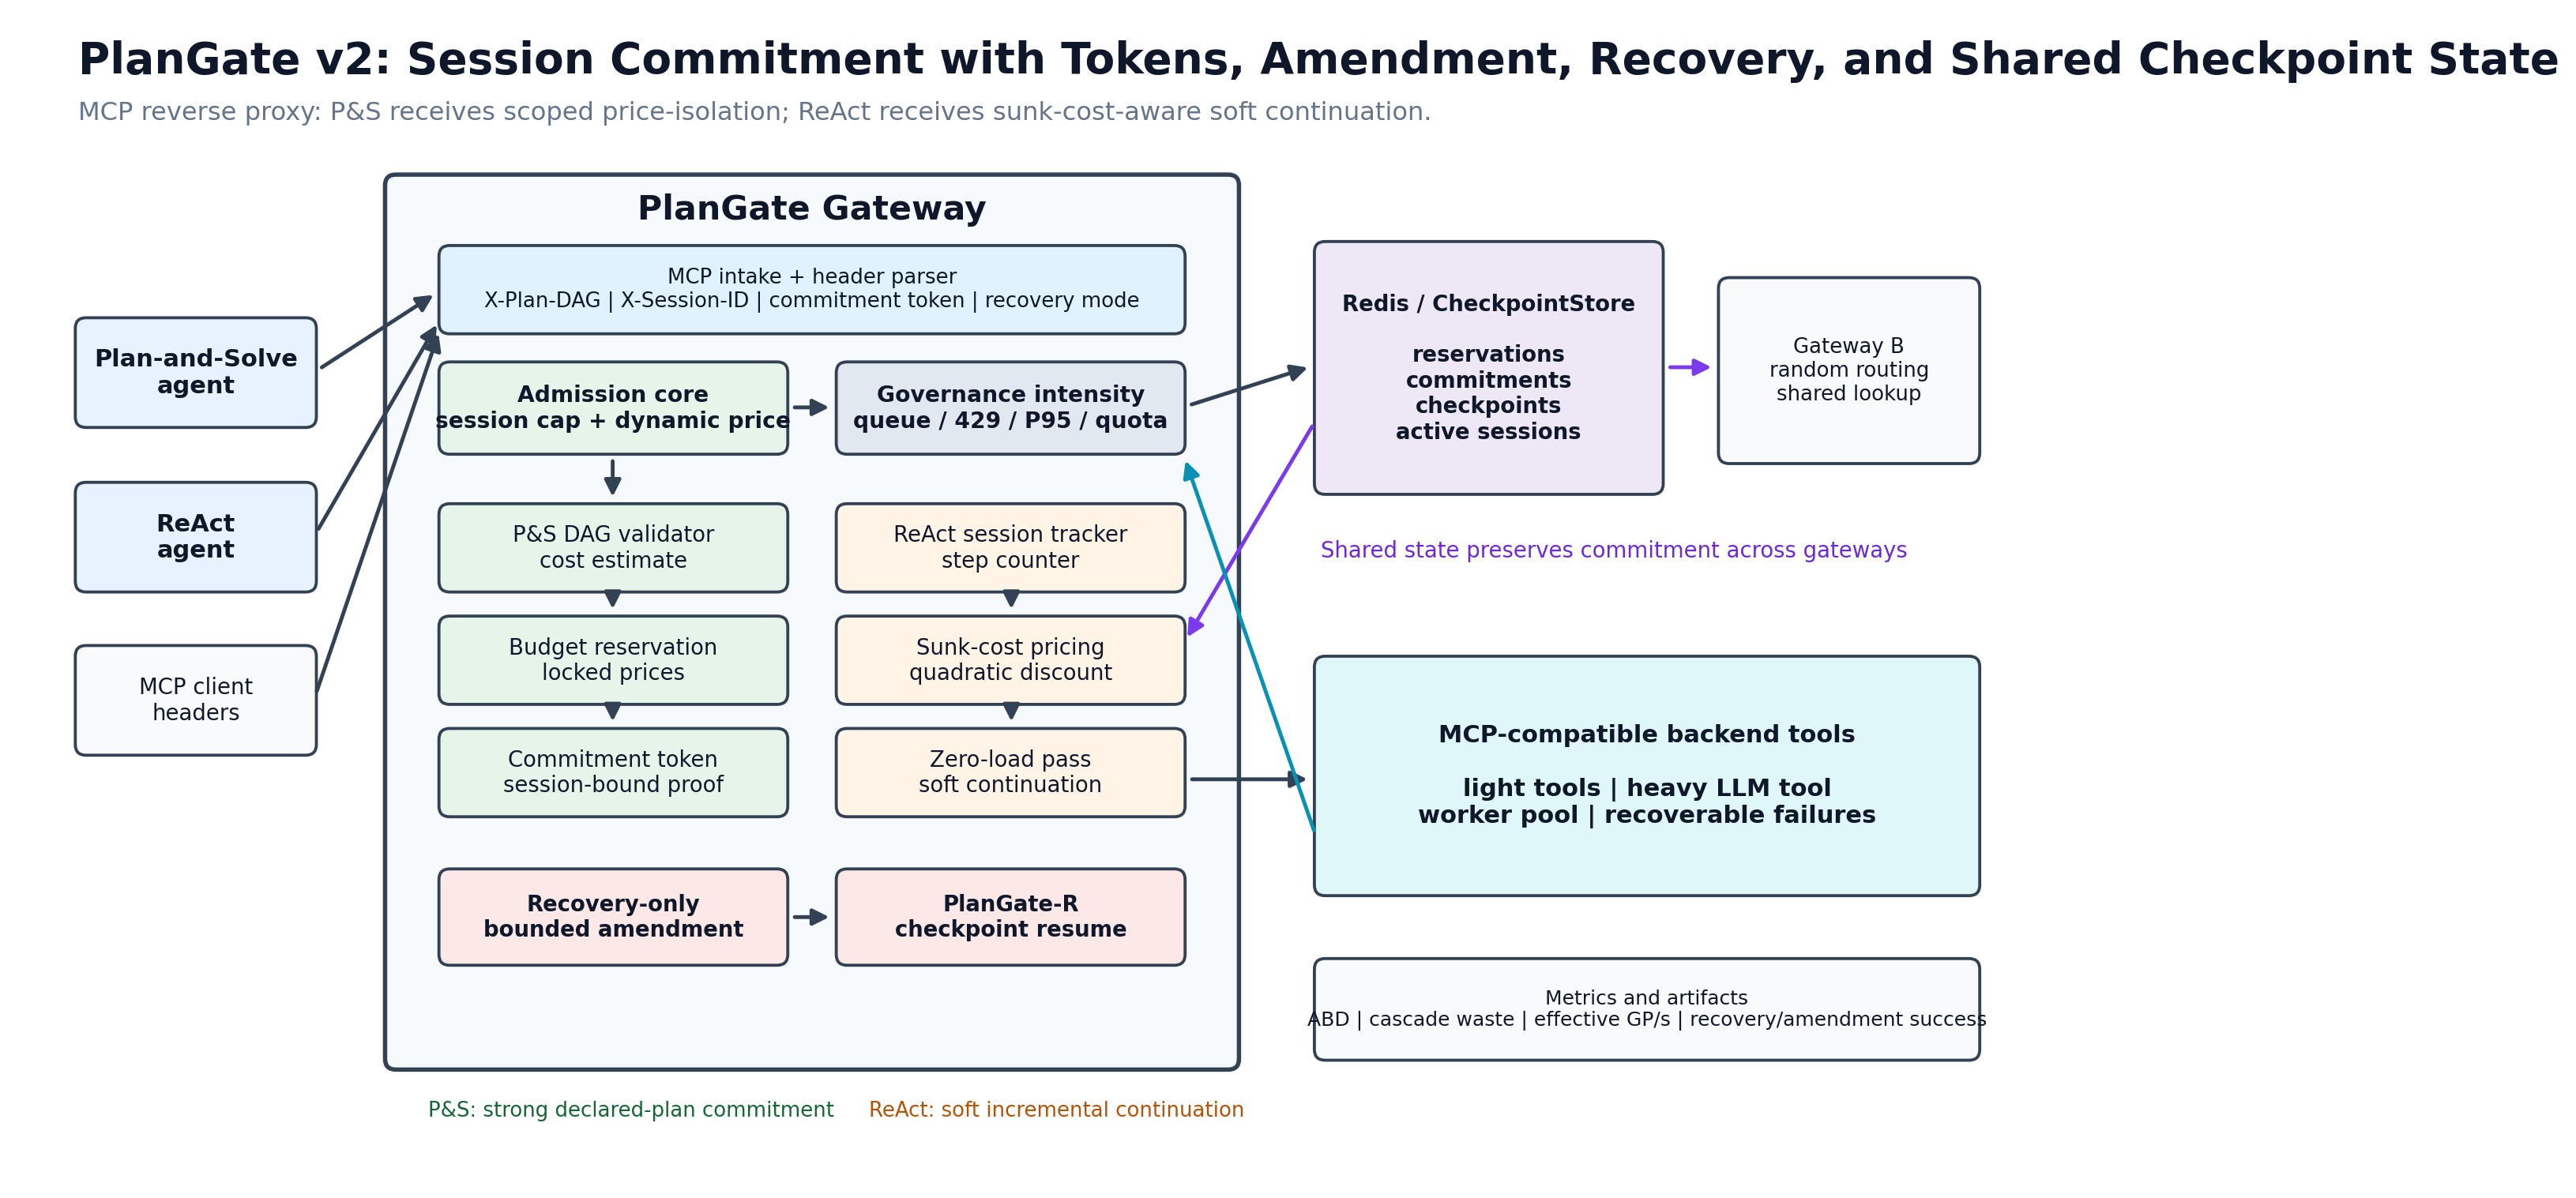
\includegraphics[width=0.96\textwidth]{architecture.png}
\caption{
PlanGate architecture overview. PlanGate separates session-level admission and commitment from per-request MCP routing. P\&S sessions use atomic plan admission with budget reservation, locked prices, commitment tokens, and bounded recovery-scoped amendment; ReAct sessions use sunk-cost-aware continuation pricing. PlanGate-R provides P\&S-only checkpoint recovery. Redis-backed shared state is evaluated for reservation/checkpoint lookup in \S\ref{sec:multigateway}; replicated-store fault tolerance and ReAct distributed progress remain outside this paper.
}
\label{fig:arch}
\end{figure*}

The gateway's request routing is header-driven and operates in constant time per request. Upon receiving a \texttt{tools/call} request, the gateway inspects three HTTP headers to determine the governance mode:


\noindent\textbf{Case 1: \texttt{X-Plan-DAG} present.} The request is the first step of a P\&S session. The gateway extracts the full DAG, validates it via topological sort, computes the total price, and performs atomic admission (\S\ref{sec:preflight}).

\noindent\textbf{Case 2: \texttt{X-Session-ID} present, session has budget reservation.} The request is a subsequent step of an admitted P\&S session. The gateway retrieves the locked price snapshot and bypasses real-time load shedding (\S\ref{sec:budget}).

\noindent\textbf{Case 3: \texttt{X-Session-ID} present, no reservation.} The request belongs to a ReAct session. If the session is new (step 0), the gateway performs relaxed admission with a session capacity check. If the session is continuing (step $K \geq 1$), sunk-cost-aware pricing is applied (\S\ref{sec:sunkcost}).


\subsection{Pre-flight Atomic Admission}
\label{sec:preflight}

When a P\&S agent submits a DAG plan, PlanGate performs \emph{pre-flight atomic admission}: a single step-zero decision that determines whether the entire session can proceed. The DAG is represented as a set of steps $\{s_1, s_2, \ldots, s_n\}$, each specifying a tool name $t_i$ and dependencies. The gateway computes the total cost:

\begin{equation}
C_{\text{total}} = \sum_{i=1}^{n} P_{\text{eff}}(t_i), \quad P_{\text{eff}}(t) = P_{\text{own}} \times w_t
\end{equation}

\noindent where $P_{\text{own}}$ is the gateway's current self-price (reflecting backend load) and $w_t$ is the tool-specific weight multiplier (heavy tools like LLM inference have $w_t > 1$). The summation estimates total committed work for budget sufficiency. A Rajomon-style maximum price can be used as a separate bottleneck or peak-capacity signal, but it does not replace the total reservation cost when all declared steps must execute. If the agent's declared budget $B < C_{\text{total}}$, the entire session is rejected at step zero---before any tool execution occurs. This prevents price-induced cascading waste for P\&S sessions whose plans accurately reflect their execution and whose reservations remain valid.


After price validation, the request is gated by a \emph{session capacity semaphore} implemented as a buffered Go channel of size $M$. If the channel is full, the request queues for up to $W$ duration (configurable) before being rejected. This provides back-pressure at the session level rather than the request level, preventing the gateway from admitting more sessions than it can sustain.


\subsection{Budget Reservation}
\label{sec:budget}

Upon successful pre-flight admission, PlanGate creates a \emph{budget reservation} for the session. This reservation captures a snapshot of the current effective price for each tool in the DAG:

\begin{equation}
\text{LockedPrices}[t_i] = P_{\text{eff}}(t_i) \big|_{\text{admission time}}
\end{equation}

Subsequent steps in the session bypass the real-time load shedding mechanism entirely: they use the locked price, not the current market price. This design provides two properties:


\noindent\textbf{Isolation property:} An admitted session's execution is immune to price increases caused by other sessions arriving after admission. This prevents the scenario where a session passes step-0 admission but fails at step 5 because 50 new sessions arrived and drove the price up.

\noindent\textbf{Budget sufficiency:} If a session's budget covers the total cost at admission time, the locked-price reservation remains sufficient for all subsequent declared steps, preventing price-induced rejection within the declared plan scope, assuming reservation validity, backend availability, and plan accuracy.


Reservations have a configurable TTL and are garbage-collected by a background goroutine every 30 seconds. When a reservation expires or is released, the session capacity slot is returned to the semaphore, allowing new sessions to be admitted.

\textbf{Boundary Conditions.}
Three edge cases: (1)~\emph{TTL expiry:} the session falls back to sunk-cost-discounted market prices (ReAct mode). (2)~\emph{Agent crash:} the reservation is garbage-collected and the session slot released. (3)~\emph{Budget exactly equals cost:} admitted with $\epsilon{=}10^{-9}$ floating-point tolerance.

\textbf{Plan Drift and DAG Mismatch Handling.}
Budget-reserved commitments protect against \emph{price-induced} mid-session rejection but do not provide unconditional completion guarantees. Three classes of plan deviation are handled explicitly:
(1)~\emph{Invalid DAG:} If the submitted DAG fails topological-sort validation (e.g., cycles, unknown tool names), the session is rejected at step~0 with a descriptive error code before any compute is consumed.
(2)~\emph{Plan drift (extra steps):} If a P\&S agent exceeds its declared step count---e.g., because intermediate results prompt additional tool calls---the reservation expires at the declared boundary, and subsequent steps are governed under sunk-cost-discounted ReAct pricing. This graceful degradation preserves the invested compute while subjecting undeclared work to current-load admission.
(3)~\emph{Undeclared tool substitution:} If an agent invokes a tool not present in its declared DAG, the call is priced at current market rate (no locked-price benefit) but is not automatically rejected, allowing the session to complete at higher cost.
These semantics ensure that budget reservation provides scoped price-isolation protection within its declared scope while degrading gracefully---rather than failing catastrophically---when plans diverge from declarations. The scope of the budget-reserved commitment is thus: protection against price volatility and admission-wave interference for the declared plan, \emph{not} an unconditional completion guarantee against all failure modes (e.g., backend crashes, tool errors, or plan inaccuracy).

\subsection{Commitment Tokens, Amendment, and Checkpoint State}
\label{sec:commitment-tokens}

The implementation exposes commitment as an explicit protocol object rather than only an internal gateway decision. When a P\&S session is admitted, PlanGate returns a commitment token bound to the session identifier, declared plan, locked reservation metadata, and gateway secret. Subsequent amendment and recovery operations must present this token, which prevents an unauthenticated client from converting an ordinary request into protected continuation work. In the artifact implementation, commitment can be disabled for ablation with \texttt{--commitment-token-mode off}; otherwise it is optional for ordinary continuation and required for amendment paths.

PlanGate also supports bounded plan amendment for a narrow failure mode: a plan-accurate P\&S session reaches a recoverable interruption or plan-boundary mismatch, and the client submits a small delta plan rather than restarting the whole task. The evaluated configuration uses \texttt{--plan-amendment-mode recovery-only}, requires a valid commitment token, allows at most three amendments per session, and allows no positive budget delta. Thus amendment is not a general re-planning engine; it is a controlled mechanism for preserving committed prefix work when a declared plan needs a small recovery-scoped correction.

Finally, reservation, recovery, and amendment metadata are stored through a \texttt{CheckpointStore} abstraction. Local experiments use the in-memory store to isolate mechanism behavior. The CloudLab validation uses Redis-backed state so that randomly routed continuation requests can find the same reservation/checkpoint metadata across gateways. This split is important for interpretation: the core mechanism is session commitment, while Redis is the deployment substrate that preserves commitment semantics when a session crosses gateway processes.

\subsection{Sunk-Cost-Aware Dynamic Pricing for ReAct}
\label{sec:sunkcost}

ReAct agents cannot provide a plan upfront, so PlanGate cannot perform pre-flight atomic admission. Instead, it applies \emph{sunk-cost-aware dynamic pricing}: the effective admission price decreases as the session progresses, reflecting the increasing cost of rejection.


\textbf{Step 0 (First Call):} The session is new and has zero invested compute. PlanGate applies the full admission price, modulated by a joint intensity-load signal:

\begin{equation}
\label{eq:step0}
P_{\text{step0}} = P_{\text{base}} \times I(t) \times L(t)
\end{equation}

\noindent where $P_{\text{base}}$ is a configurable reference price, $I(t) \in [0, 1]$ is the governance intensity (from the intensity tracker), and $L(t) = N_{\text{active}} / M$ is the gateway load ratio (active sessions divided by session capacity). The product $I \times L$ creates a \emph{3D pricing surface}: the step-0 price is high only when \emph{both} the backend is stressed and the gateway is near capacity. This dual gating prevents over-rejection when only one signal indicates pressure.


\textbf{Step $K \geq 1$ (Sunk-Cost Discount):} For sessions that have already completed $K$ steps, PlanGate computes a discounted effective price:

\begin{equation}
\label{eq:sunkcost}
P_K = \frac{P_{\text{eff}} \times I(t)}
{1 + K^2 \cdot \alpha_{\text{eff}}}, 
\quad 
\alpha_{\text{eff}} = \alpha \bigl(1+\beta(1-I(t))\bigr)
\end{equation}

\noindent where $P_{\text{eff}}$ is the current effective price (with $P_{\text{base}}$ as fallback when $P_{\text{own}} = 0$), $\alpha$ is the sunk-cost coefficient, and $\beta$ controls load-dependent slack amplification. We use $\beta{=}1$ by default, which recovers the original $\alpha(2-I(t))$ form and bounds $\alpha_{\text{eff}}\in[\alpha,2\alpha]$. The quadratic term $K^2$ provides aggressive discounting: at $K=3$ with $\alpha=0.4$, $\beta=1$, and $I=1.0$, the discount factor is $1/(1+3.6)=0.22$, reducing the price to 22\% of the base. The load-modulated $\alpha_{\text{eff}}$ provides \emph{stronger discounts when load is lighter}: at $I=0.5$ and $\beta=1$, $\alpha_{\text{eff}}=1.5\alpha$, giving continuing sessions 50\% more protection. A sensitivity sweep over $\beta\in\{0,0.5,1,2,3\}$ confirms that this constant is not brittle; completion counts remain unchanged and only small cascade/fairness tradeoffs appear in Supplementary Material, Section~3.


\textbf{Zero-Load Free Pass:} When intensity $I < 0.01$---indicating no backend pressure---all continuing sessions ($K \geq 1$) pass unconditionally regardless of token balance. This optimization eliminates unnecessary price computation under light load and ensures that PlanGate degrades to a simple pass-through when the system is idle.


\textbf{Unified admission logic.}
For every \texttt{tools/call}, PlanGate first reads the backend intensity $I(t)$ and gateway load ratio $L(t)=N_{\text{active}}/M$, then dispatches to one of three paths. If \texttt{X-Plan-DAG} is present at step~0, PlanGate validates the DAG, computes $C_{\text{total}}$, checks the declared budget, acquires a session slot, and creates a locked-price reservation. If a later request has \texttt{X-Session-ID} and a valid reservation, PlanGate uses the locked prices and bypasses real-time load shedding for the declared plan. Otherwise, the request is treated as ReAct: step~0 uses Eq.\,(3), continuing steps use Eq.\,(4), and $I(t)<0.01$ triggers a zero-load free pass.

\textbf{Commitment semantics: P\&S vs.\ ReAct.}
P\&S sessions receive strong atomic admission and temporal isolation within the declared plan, so continuation discounting is unnecessary. ReAct sessions receive relaxed step-0 admission and no temporal isolation, but sunk-cost discounting makes mid-session rejection increasingly unlikely as invested compute grows. These intentionally different guarantees reflect the different information available at admission time.

\subsection{Governance Intensity Tracking}

PlanGate uses two implementations of the \texttt{IntensityProvider} interface to compute governance intensity $I(t) \in [0, 1]$:

\noindent\textbf{GovernanceIntensityTracker} (mock workloads): Derives intensity from the gateway's internal queuing delay price. It normalizes $P_{\text{own}}$ against a reference maximum and applies hysteresis gating to prevent oscillation.

\noindent\textbf{ExternalSignalTracker} (real LLM): Fuses three external API signals via weighted EMA. Signal weights: 429 rate ($w=0.5$), latency P95 ($w=0.3$), and RateLimit-Remaining ($w=0.2$). The tracker uses hysteresis gating with separate activation ($>0.15$ for 3 consecutive cycles) and deactivation ($<0.05$ for 10 consecutive cycles) thresholds.

\textbf{External API Error Handling.}
HTTP 429 responses from external providers increment the 429-rate counter, directly increasing governance intensity $I(t)$ and tightening admission. HTTP 5xx responses are treated as transient provider failures that contribute to cascade waste accounting but do \emph{not} trigger admission tightening, since provider outages are not addressable by client-side throttling.


The raw score is computed via dynamic-weight normalization: only signals with non-zero data contribute to the weighted average, preventing inactive dimensions from diluting the score:

\begin{equation}
S_{\text{raw}} = \frac{\sum_{d \in \mathcal{D}_{\text{active}}} w_d \cdot s_d}{\sum_{d \in \mathcal{D}_{\text{active}}} w_d}
\end{equation}

\noindent where $\mathcal{D}_{\text{active}} \subseteq \{429, \text{latency}, \text{rateLimit}\}$ is the set of dimensions with available data, $w_d$ is the dimension weight, and $s_d \in [0,1]$ is the normalized signal value.

\subsection{Dynamic Pricing Engine}

PlanGate employs a queuing-delay-based dynamic pricing engine. The base price $P_{\text{own}}$ is updated periodically based on observed queuing delay:

\begin{equation}
P_{\text{own}}(t+1) = \begin{cases}
P_{\text{own}}(t) + K_p \cdot \Delta_q & \text{if } \Delta_q > 0 \\
P_{\text{own}}(t) - D_{\text{step}} & \text{if } \Delta_q \leq 0
\end{cases}
\end{equation}

\noindent where $\Delta_q = \text{observedDelay} - \text{latencyThreshold}$ is the queuing delay gap, $K_p$ is the proportional gain, and $D_{\text{step}}$ is the decay step. When using the exponential decay strategy, the price increase is amplified by $2^{c}$ where $c$ is the count of consecutive increases.


PlanGate extends this engine with: (a)~\emph{tool weights} that multiply the base price for heavy tools, creating differentiated pricing; (b)~an \emph{adaptive profile system} that detects load regime transitions (idle/stable/volatile/spike) and hot-swaps parameter sets; and (c)~\emph{moving-average smoothing} to filter short-term latency noise from pricing decisions.

\subsection{Practical Abuse Control}
\label{sec:abuse-control}

PlanGate's admission control uses client-declared metadata (\texttt{X-Total-Budget}, \texttt{X-Plan-DAG}), so the gateway maintains a lightweight per-agent trust score to discourage inflated budgets and fraudulent DAGs. Each agent starts with optimistic trust ($T_a{=}1$); successful sessions keep trust high, while budget or DAG violations reduce it. Low-trust agents have their declared budgets scaled down, and agents below a ban threshold are rejected with HTTP~403. This mechanism is intentionally simple---not a full Sybil-resistant identity system, but it prevents naive slot monopolization while keeping the admission hot path inexpensive. Complete implementation details (EWMA trust update rule, enforcement thresholds, flat violation penalty) and the adversarial robustness experiment ($2.5\times$ success count of NG with 1.0 cascade failure under 10\% adversarial injection) appear in Supplementary Material, Section~4. This mechanism is not part of the core session-commitment abstraction; it is a practical guardrail against naive metadata abuse.

\subsection{Continuation Discount Rationale}
\label{sec:discount-rationale}

This section provides a lightweight rationale for the shape of PlanGate's ReAct continuation discount. The goal is not to model the queue exactly, but to explain why the discount should become increasingly aggressive as sunk compute grows. Consider a session of $N$ uniform-cost steps. With per-request pricing, a rejection at step $k$ wastes $k$ completed steps, so the expected waste scales as $O(N^2)$ for small rejection probability. A continuation discount $d(k)$ lowers the rejection probability of later steps to reflect sunk cost. Linear discounts reduce the order to $O(N)$, while the quadratic discount $d(k)=1/(1+k^2\alpha)$ yields logarithmic waste, $O(\ln N)$, under the same simplified assumptions. Budget reservation for plan-accurate P\&S sessions is the limiting case: within the declared plan scope, and assuming reservation validity plus backend availability, price-induced rejection is removed from continuing steps.
For $N\in[3,10]$ and $\alpha{=}0.5$, the exact sum $\sum_k k/(1+0.5k^2)$ gives a $2.3\times$ to $12.0\times$ waste reduction over per-request pricing. This motivates the design hierarchy used by PlanGate: budget-reserved scoped protection for P\&S agents when a plan is known, and quadratic sunk-cost discounting for ReAct agents when future steps are unknown. Section~\ref{sec:discountablation} empirically compares quadratic, linear, exponential, and logarithmic discounts. The complete formal proof---including Claim~1 (waste reduction ratio), integral upper-bound derivation, and $O(\ln N/\alpha)$ confirmation---appears in Supplementary Material, Section~2.

\subsection{Checkpoint-Aware Recovery Extension (PlanGate-R)}
\label{sec:recovery-ext}

PlanGate provides admission integrity: it prevents governance-induced mid-session failures by ensuring that an admitted, correctly-priced session is not ejected by price pressure, load shedding, or session-cap eviction.
An orthogonal failure mode exists, however: an already-admitted P\&S session may still be interrupted by a recoverable transient backend failure that is not caused by the governance policy.
Under naive retry, the session restarts from step~0, discarding all completed prefix work.
PlanGate-R is a checkpoint-aware extension that complements base session commitment by handling this specific case.

\textbf{Mechanism.}
After each successful tool-call step, PlanGate-R saves a lightweight checkpoint recording the completed step index, step metadata, and the remaining declared plan.
When a later step returns a recoverable failure classification (\texttt{RecoveryDecisionRecoverable}), the checkpoint is marked as recovery-eligible.
A resume request---identified by an \texttt{X-Recovery-Mode: resume} header---can then re-enter the execution path at the first uncompleted step; completed prefix steps are not replayed.
The existing session reservation and \texttt{X-Session-ID} are reused for the resumed execution.

\textbf{Design boundary.}
The current prototype has four explicit scope limits:
(1)~P\&S sessions only---ReAct sessions expose no pre-declared DAG against which to verify prefix soundness, so checkpoint-based recovery is not applicable;
(2)~store-dependent durability---the in-memory store used in local mechanism tests is not durable, while Redis-backed CloudLab runs validate cross-node lookup but not replicated-store fault tolerance;
(3)~no semantic re-planning---the resume path re-executes the declared DAG plan, not a re-reasoned one;
(4)~multi-tenant scheduling between recovery and fresh sessions is not formally evaluated in this paper, though the prototype includes quota logic to bound concurrent recoveries.
PlanGate-R reduces per-session replay waste within declared P\&S plan scope; it does not provide completion guarantees beyond those of base session commitment.

\section{Implementation}

PlanGate is implemented in approximately 3,500 lines of Go (gateway and governor) and 2,000 lines of Python (backend, agents, and evaluation scripts).
\textbf{Gateway.} The PlanGate gateway is built on Go's \texttt{net/http} package, using goroutines for concurrent request handling. Session capacity is implemented as a buffered channel (\texttt{chan struct\{\}}), leveraging Go's channel semantics for lock-free semaphore behavior. The price table uses \texttt{sync.Map} for concurrent read/write access. The budget reservation manager uses \texttt{sync.Map} for O(1) session lookup with a background cleanup goroutine running every 30 seconds. Cross-compilation targets Linux/amd64 with \texttt{CGO\_ENABLED=0} for static binary deployment.


\textbf{MCP Backend.} The Python backend registers 10 tools (5 real tools for LLM mode, 5 mock tools for controlled experiments) and serves them via HTTP/JSON-RPC. Mock tools simulate configurable latency distributions (sub-millisecond to 150\,ms for light tools; 800\,ms base latency plus congestion penalty, upper bound $\approx$2800\,ms for heavy tools) using \texttt{time.sleep}; they encompass two qualitatively distinct latency regimes (I/O-bound lightweight: calculator, weather query, web fetch, text formatter; compute-bound heavyweight: document embedding, code sandbox, LLM inference stub) that together span the full governance-relevant spectrum. Real tools proxy to external APIs (GLM-4-Flash, web search) with signal collection for the ExternalSignalTracker. Note that PlanGate's governance is \emph{tool-agnostic}: admission decisions depend only on tool name-to-weight mappings ($w_t$), not on tool content or count. A production deployment with hundreds of tools would map each to the same weight-tier classification; the governance algorithm and commitment semantics remain unchanged.


\textbf{Evaluation Infrastructure.} The test harness manages experiment lifecycle: building the Go gateway, launching the Python backend, generating load via concurrent agent clients, and collecting per-session and per-step metrics. Each experiment runs multiple times to control for variance. CPU isolation is enforced via \texttt{taskset}: cores 0--3 for load generation, 4--7 for the gateway, and 8--15 for the backend.



% 5. EVALUATION
\section{Evaluation}

\subsection{Experimental Setup}

We evaluate PlanGate on an Intel Core i7-12700H workstation with Go~1.25.6 and Python~3.10.12, and supplement the local results with CloudLab and provider-backed smoke evidence. We compare against request-level and session-level baselines: No Governance (NG), Static Rate Limit (SRL; \texttt{qps=65}, \texttt{burst=400}, \texttt{max\_conc=55}), Rajomon with its best-case \texttt{price\_step=5}, Rajomon+SB (Rajomon with session bookkeeping), SBAC (\texttt{max\_sessions=150}), Progress-Priority (PP; \texttt{max\_sessions=150}), and PlanGate ablations. PlanGate Full uses \texttt{price\_step=40}, \texttt{max\_sessions=30}, quadratic discounting with $\alpha{=}0.5$ and $\beta{=}1$, commitment tokens in optional mode, recovery enabled, and recovery-only plan amendment unless stated otherwise.

Our primary metric is \emph{admitted-but-doomed rate} (ABD): the fraction of admitted sessions that fail mid-execution. We also report task success rate, effective goodput (GP/s), raw goodput, step-0 rejections, cascade waste, recovery success, amendment success, and commitment-token issuance. Table~\ref{tab:commitment-quality} uses a 200-session, 50/s-arrival, 200-concurrency mixed P\&S/ReAct workload to measure mode-stratified ABD. Core mock experiments use 500 sessions at 50/s arrival and up to 200 concurrency; parameter sweeps use 200 sessions at 15/s arrival and 20 concurrency unless stated otherwise. P\&S sessions issue 3--7 tool calls, ReAct sessions issue 1--7 tool calls, and tools are classified into light ($<150$\,ms, weight~1) and heavy (800\,ms base plus congestion penalty, weight~5) classes. Mock results average 5 independent runs unless otherwise stated.

The evaluation follows an evidence hierarchy rather than a single headline benchmark: \emph{Tier~1} (\S\ref{sec:commitment_quality}--\S\ref{sec:bursty_longtail}) uses controlled mock workloads with hard capacity limits; \emph{Tier~2} (\S\ref{sec:new-mechanism-ablation}, \S\ref{sec:recovery-eval}) isolates the new commitment/amendment/recovery mechanisms under local failure workloads; \emph{Tier~3} (\S\ref{sec:multigateway}) validates Redis-backed shared state under cross-gateway routing; \emph{Tier~4} (\S\ref{sec:reallm}--\S\ref{sec:selfhosted}) treats provider-backed and self-hosted LLM runs as boundary and smoke evidence. A throughput--latency summary (\S\ref{sec:tput_latency}) consolidates Exp1/Exp5/Exp6/Exp10 raw and effective goodput. The 10-tool setup is intentionally small but cost-diverse: PlanGate's decisions depend on per-tool weights and session length, not the total number of registered tools.

\subsection{Commitment Quality: The Core Result}
\label{sec:commitment_quality}

\input{table_commitment_quality_submission}

Table~\ref{tab:commitment-quality} presents the central experimental result: PlanGate's commitment quality advantage is statistically significant against the comparison systems shown in the table ($p < 0.01$ for ABD\textsubscript{total}, ABD\textsubscript{P\&S}, ABD\textsubscript{ReAct}, and GP/s via permutation test). PG-noRes is an internal ablation, not an external baseline.

\textbf{Budget-reserved commitment for P\&S sessions.} PlanGate observes ABD\textsubscript{P\&S}$\,{=}\,$0.0\% across all 5 controlled mock runs---within declared plan scope, valid reservations, available backends, and plan-accurate P\&S execution. Under those conditions, budget reservation prevents price-induced mid-session rejection within the declared plan scope. The necessity of this mechanism is demonstrated by PG-noRes, a PlanGate variant without budget reservation, which suffers ABD\textsubscript{P\&S}$\,{=}\,$81.6\%. PG-noRes is not a generic ablation but a specific test of whether \emph{temporal isolation} (price locking) is required for budget-reserved commitments; the answer is unambiguous.

\textbf{Soft commitment for ReAct sessions.} PlanGate achieves ABD\textsubscript{ReAct}$\,{=}\,$21.7\%, compared to 54--65\% for session-based baselines (SBAC, PP) and 61--66\% for per-request pricing baselines (Rajomon, Rajomon+SB). Since ReAct sessions cannot declare plans upfront, price-isolation protection is unavailable; instead, sunk-cost-aware discounting provides a \emph{continuation incentive} that substantially reduces mid-execution abandonment. This is an inherently weaker guarantee than P\&S budget reservation---reflecting the fundamental information asymmetry between the two agent types.

\textbf{Structural conclusions.}
Three pairwise comparisons isolate the contributions of individual mechanisms:
\begin{enumerate}[nosep,leftmargin=*]
  \item \emph{Session bookkeeping $\neq$ session commitment}: Rajomon$\,{\approx}\,$Rajomon+SB (ABD 65.4\% vs.\ 64.7\%). Adding session tracking to per-request pricing does not improve commitment quality because the pricing model itself is session-oblivious.
  \item \emph{Progress favoritism $\neq$ commitment}: PP$\,{\approx}\,$SBAC (ABD 62.9\% vs.\ 56.0\%). Prioritizing sessions with more completed steps does not substitute for explicit sunk-cost discounting.
  \item \emph{Reservation is necessary}: PG-noRes vs.\ PlanGate (ABD\textsubscript{P\&S} 81.6\% vs.\ scoped 0.0\% under controlled mock assumptions). Without budget reservation, even PlanGate's other mechanisms cannot deliver budget-reserved commitments.
\end{enumerate}

\textbf{Goodput.} PlanGate's GP/s (50.4$\pm$6.2) is 97\% higher than Rajomon's best-case (25.5$\pm$4.3) and 56\% higher than SBAC (32.3$\pm$2.2), because fewer admitted sessions are wasted on cascading failures.

\textbf{Session-cap fairness.}
SBAC and PP use \texttt{max\_sessions=150} (their default configurations), while PlanGate uses \texttt{max\_sessions=30}. To verify that PlanGate's ABD advantage is not simply a cap artifact, we highlight two controls.
\emph{First}, PG-noRes shares PlanGate's exact cap (\texttt{max\_sessions=30}) and pricing but disables budget reservation, yet suffers ABD\textsubscript{P\&S}$\,{=}\,$81.6\%---ruling out admission conservatism as the explanation.
\emph{Second}, a supplementary SBAC run at \texttt{max\_sessions=30} achieves ABD$\,{\approx}\,$0.6\% by eliminating contention among admitted sessions, but admits only 33 of 200 total sessions; PlanGate admits 43 sessions at the same cap because pricing-driven turnover recycles slots faster, yielding 5.5\% more successful completions (34.6 vs.\ 32.8). The governance mechanism---not the cap value---determines commitment quality.


\subsection{Rajomon Sensitivity Analysis}
\label{sec:rajomon_sens}

To ensure baseline fairness, we sweep Rajomon's \texttt{price\_step} parameter across $\{5, 10, 20, 50, 100\}$ (5 repeats each). The following table summarizes the results:

\begin{table}[h]
\centering
\small
\resizebox{\columnwidth}{!}{%
\begin{tabular}{@{}rrrr@{}}
\toprule
\textbf{Price Step} & \textbf{ABD\textsubscript{total}\%} & \textbf{SuccRate\%} & \textbf{GP/s} \\
\midrule
5   & 64.4$\pm$4.4  & 11.8 & 25.4 \\
10  & 72.2$\pm$10.5 &  9.5 & 18.4 \\
20  & 89.0$\pm$2.3  &  3.7 &  5.1 \\
50  & 89.0$\pm$3.9  &  2.8 &  7.0 \\
100 & 89.7$\pm$1.1  &  2.4 &  6.1 \\
\bottomrule
\end{tabular}}
\end{table}

The best-case configuration (\texttt{price\_step=5}) achieves ABD$\,{=}\,$64.4\%, comparable to No Governance (65.5\%)---pricing is too weak to reject overload, providing minimal session-level differentiation. At higher price steps (\texttt{price\_step$\,{\geq}\,$20}), ABD exceeds 89\% because per-request pricing ejects mid-session requests too aggressively. Neither extreme provides session commitment. We use the best-case (\texttt{price\_step=5}) in all subsequent Rajomon comparisons. This demonstrates a \emph{systematic mismatch}: per-request pricing does not account for the sequential dependencies within multi-step sessions, leaving sessions vulnerable to mid-execution ejection regardless of parameter tuning.

\begin{figure}[t]
\centering
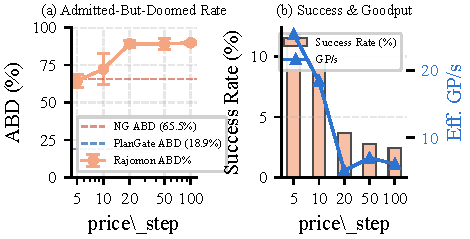
\includegraphics[width=0.9\columnwidth]{rajomon_sensitivity}
\caption{Rajomon sensitivity sweep. (a)~ABD increases monotonically with \texttt{price\_step}, never approaching PlanGate's 18.9\%. (b)~Success rate and goodput decline sharply at aggressive settings. Per-request pricing provides no session-level sweet spot.}
\label{fig:rajomon_sens}
\end{figure}

\subsection{Core Mock Performance Comparison}
\label{sec:exp1}

This experiment evaluates scoped price-induced cascade prevention and effective goodput under controlled mock conditions. The primary metrics are cascade failure count, effective GP/s, and median/tail latency.

\begin{table}[t]
\caption{Core mock performance (500 sessions, 200 concurrency, averaged over 5 runs).}
\label{tab:exp1}
\small
\resizebox{\columnwidth}{!}{%
\begin{tabular}{@{}lrrrrrr@{}}
\toprule
\textbf{Gateway} & \textbf{Succ.} & \textbf{Rej.} & \textbf{Casc.} & \textbf{Eff.GP/s} & \textbf{P50} & \textbf{P95} \\
\midrule
NG        & 28.2  & 308.4 & 163.4 & 16.3  & 1016  & 1984 \\
SRL       & 43.2  & 314.0 & 142.8 & 24.9  & 1015  & 1913 \\
SBAC      & 68.8  & 383.6 & 47.6  & 45.4  & 371   & 1379 \\
\textbf{PlanGate} & \textbf{84.4} & \textbf{415.4} & \textbf{0.2} & \textbf{54.8} & \textbf{3.6} & \textbf{864} \\
\bottomrule
\end{tabular}}
\end{table}

Table~\ref{tab:exp1} shows the refreshed core mock result averaged over 5 runs. PlanGate observes near-zero price-induced cascade failures (0.2 per run) under controlled mock conditions, valid reservations, available backends, and plan-accurate P\&S execution, while NG averages 163.4 cascade failures per run and SRL averages 142.8. PlanGate's effective goodput (54.8~GP/s) is $3.4\times$ that of NG (16.3~GP/s) and $2.2\times$ that of SRL (24.9~GP/s). Even compared to SBAC---the best session-aware baseline at 45.4~GP/s---PlanGate achieves a $1.2\times$ improvement.


The cost of PlanGate's cascade protection is a higher step-0 rejection rate: PlanGate rejects an average of 415 sessions at step 0, compared to 308 for NG. However, these step-0 rejections are \emph{zero compute-waste}: no tool execution has begun. They are not zero user cost, because rejected users still experience reduced availability or must retry later. The net effect is that PlanGate converts wasteful cascade failures into clean step-0 rejections, improving resource efficiency; incorporating user utility, retry cost, and SLA-aware admission remains future work.

\begin{figure}[t]
\centering
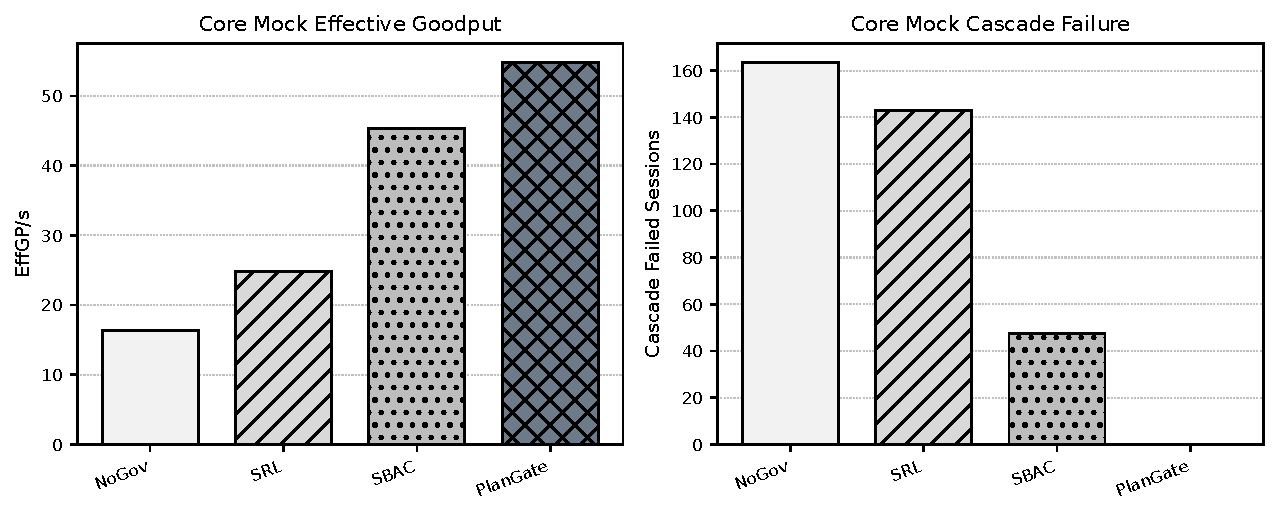
\includegraphics[width=\columnwidth]{fig_core_effgp_cascade}
\caption{Refreshed core mock evidence from the artifact package. PlanGate maintains the highest effective GP/s while reducing cascade failures to the near-zero range; the benefit is resource efficiency under hard capacity, not additional backend capacity.}
\label{fig:core_effgp_cascade}
\end{figure}
\subsection{Mechanism Ablation}
\label{sec:new-mechanism-ablation}

We separate mechanism evidence into two layers. The first refreshes the original budget/session-cap ablation; the second targets the post-P3 mechanisms---commitment tokens, amendment, and recovery---under workloads that actually exercise failure and amendment paths.

\begin{table}[t]
\caption{Budget/session-cap ablation (500 sessions, averaged over 5 runs).}
\label{tab:ablation}
\small
\resizebox{\columnwidth}{!}{%
\begin{tabular}{@{}lrrrrr@{}}
\toprule
\textbf{Variant} & \textbf{Succ.} & \textbf{Casc.} & \textbf{Eff.GP/s} & \textbf{P50} & \textbf{P95} \\
\midrule
PlanGate Full    & 88.6  & 0.0  & 56.8  & 4.2  & 881 \\
wo-BudgetLock    & 21.2  & 8.8  & 10.9  & 1.8  & 157 \\
wo-SessionCap    & 98.0  & 3.6  & 57.0  & 48.1 & 1189 \\
\bottomrule
\end{tabular}}
\end{table}

Removing budget reservation (\emph{wo-BudgetLock}) reduces effective goodput from 56.8~GP/s to 10.9~GP/s---a $5.2\times$ degradation---and introduces mid-session failures. Without price locking, sessions admitted at step~0 face escalating prices from subsequent arrivals and can fail after consuming prefix work. Removing session-cap control does not reduce mean goodput in this setting, but it raises the peak active-session boundary and leaves the system exposed under heavier concurrency; the additional cascades show why budget reservation alone is not a complete admission policy.

\begin{figure*}[t]
\centering
\begin{subfigure}[t]{0.49\textwidth}
\centering
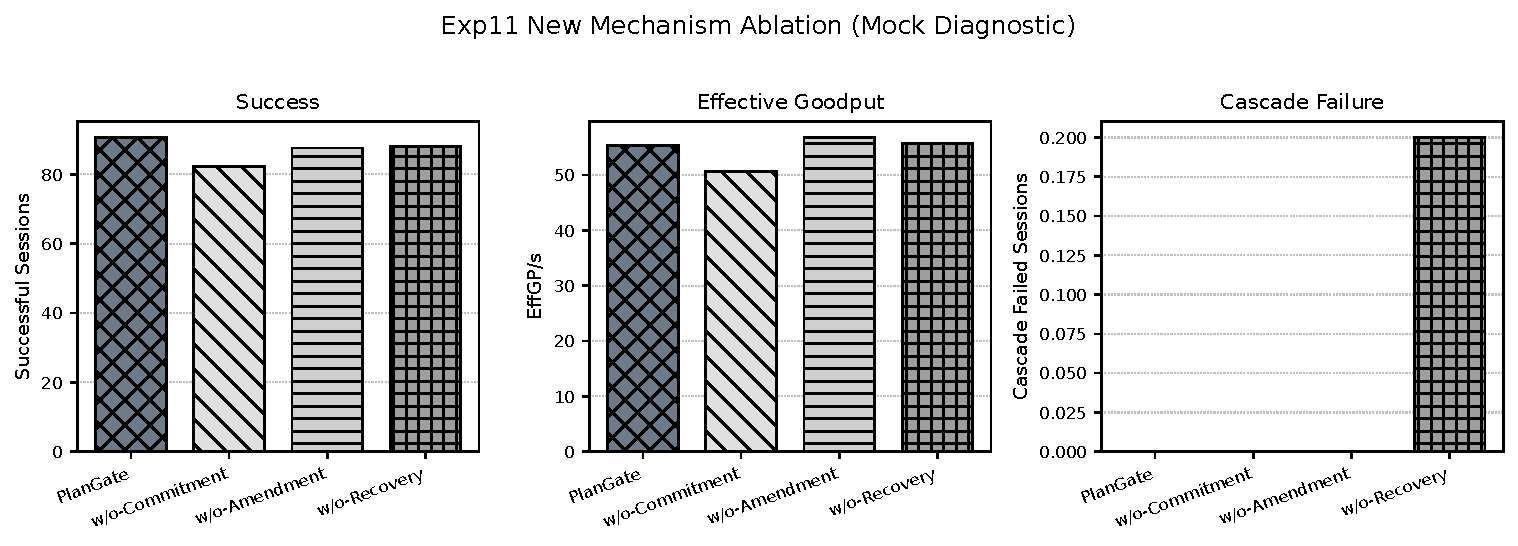
\includegraphics[width=\textwidth]{fig_exp11_new_mechanism_ablation}
\caption{Standard mock diagnostic/regression ablation.}
\label{fig:exp11_new_mech}
\end{subfigure}
\hfill
\begin{subfigure}[t]{0.49\textwidth}
\centering
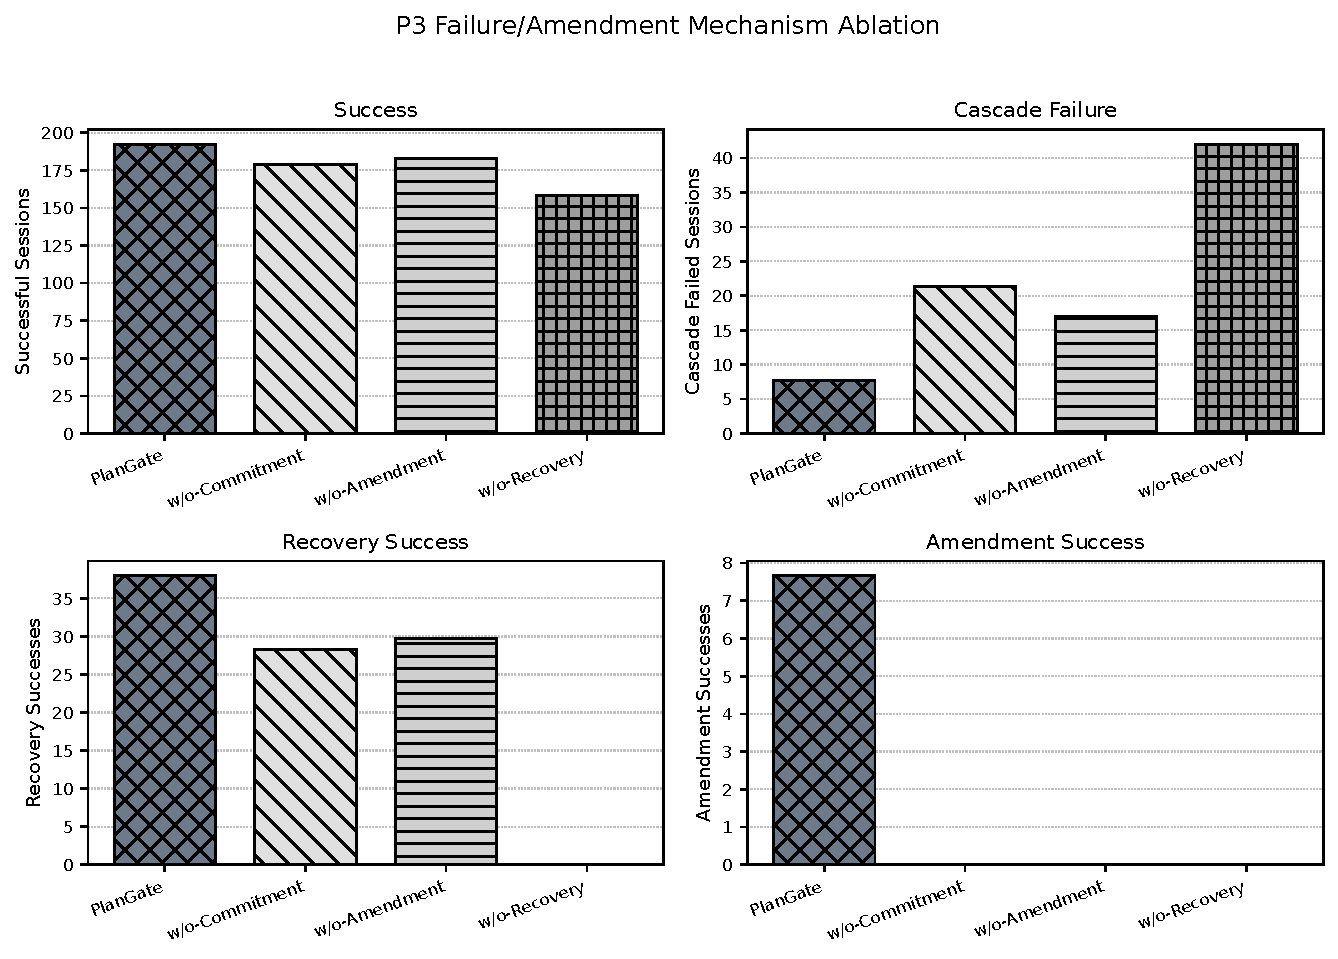
\includegraphics[width=\textwidth]{fig_p3_mechanism_ablation}
\caption{Failure/amendment workload ablation.}
\label{fig:p3_mech}
\end{subfigure}
\caption{Post-P3 mechanism ablations. The standard mock ablation checks that toggling each new mechanism does not create regressions under ordinary load. The failure/amendment ablation is the stronger signal: disabling commitment removes commitment issuance, disabling amendment drives amendment success to zero, and disabling recovery drives recovery success to zero.}
\label{fig:new_mechanism_ablation}
\end{figure*}

\begin{table}[t]
\centering
\caption{Failure/amendment mechanism ablation ($S{=}200$, $C{=}50$, failure rate 0.2, amendment rate 0.2, $N{=}3$ repeats). Values are per-run means.}
\label{tab:p3_failure_mech}
\small
\resizebox{\columnwidth}{!}{%
\begin{tabular}{@{}lrrrrr@{}}
\toprule
\textbf{Variant} & \textbf{Succ.} & \textbf{Casc.} & \textbf{Recov. Succ.} & \textbf{Amend. Succ.} & \textbf{Commit Issued} \\
\midrule
\textbf{Full}    & \textbf{192.3} & \textbf{7.7}  & \textbf{38.0} & \textbf{7.7} & \textbf{194.7} \\
wo-Commitment    & 178.7 & 21.3 & 28.3 & 0.0 & 0.0 \\
wo-Amendment     & 183.0 & 17.0 & 29.7 & 0.0 & 193.3 \\
wo-Recovery      & 158.0 & 42.0 & 0.0  & 0.0 & 196.7 \\
\bottomrule
\end{tabular}}
\end{table}

Table~\ref{tab:p3_failure_mech} isolates the semantics of the added mechanisms. Full PlanGate completes 192.3 of 200 sessions on average and records positive recovery and amendment success. Disabling commitment eliminates commitment issuance entirely and prevents amendment from being authorized. Disabling amendment preserves commitment issuance but forces amendment success to zero, increasing cascades to 17.0. Disabling recovery is the most damaging failure-specific ablation: recovery success is exactly zero and cascade failures rise to 42.0. The \emph{wo-Recovery} effective-goodput rate is not interpreted as a win because many sessions terminate early; success count and cascade-failure count are the appropriate metrics for this failure workload.
\subsection{Discount Function Ablation}
We additionally sweep the load-modulation coefficient $\beta$ in Supplementary Material, Section~3. The sweep confirms that $\beta{=}1$ is a conservative default rather than a fragile magic constant: all settings complete the same number of sessions, while larger $\beta$ values only marginally reduce cascades at the cost of slightly higher step-0 rejection or lower fairness.
\label{sec:discountablation}

A key design choice in PlanGate's sunk-cost pricing is the use of a quadratic discount function $1/(1+K^2\alpha)$. To validate this choice, we compare four discount function families: \emph{quadratic} ($K^2$), \emph{linear} ($K$), \emph{exponential} ($e^{K}-1$), and \emph{logarithmic} ($\ln(1+K)$). All variants use the same $\alpha$ and session parameters.

\begin{table}[t]
\caption{Discount function ablation (500 sessions, pure ReAct mode \texttt{ps\_ratio=0.0}, averaged over 5 runs). All functions achieve identical success (30), but differ substantially in cascade protection and goodput.}
\label{tab:discount}
\small
\resizebox{\columnwidth}{!}{%
\begin{tabular}{@{}lrrrr@{}}
\toprule
\textbf{Function} & \textbf{Casc.} & \textbf{Eff.GP/s} & \textbf{P95} & \textbf{JFI$_s$} \\
\midrule
\textbf{Quadratic} ($K^2$)    & 15.8           & 23.3          & 843  & 0.763 \\
Linear ($K$)                   & 21.0           & 23.3          & 842  & \textbf{0.776} \\
Exponential ($e^K$)            & \textbf{11.8}  & \textbf{23.7} & \textbf{827}  & 0.772 \\
Logarithmic ($\ln(1{+}K)$)    & 31.2           & 21.0          & 830  & 0.735 \\
\bottomrule
\end{tabular}}
\end{table}

Table~\ref{tab:discount} shows that \emph{aggressive} discounters outperform \emph{moderate} ones. Exponential achieves the fewest cascade failures (11.8) and highest effective goodput (23.7~GP/s), followed closely by quadratic (15.8 cascades, 23.3~GP/s). The moderate discounters---linear and logarithmic---suffer substantially more cascades (21.0 and 31.2) and lower goodput, with logarithmic worst at 21.0~GP/s. This confirms that steeper discount curves at early steps ($K{=}2,3$) provide critical protection during the mid-session window where most cascades occur.

We choose the quadratic discount ($K^2$) as the practical operating point. Exponential discounting achieves marginally fewer cascades in this experiment (11.8 vs.\ 15.8), but $K^2$ provides near-equal cascade protection while keeping the admission hot path simple---no floating-point exponential required---and remaining more predictable for deeper sessions ($K{>}10$) where $e^K$ can grow excessively permissive. The ablation should be read not as a claim of global optimality, but as evidence that aggressive convex discounts are necessary and that $K^2$ provides a stable practical tradeoff in our workload. 
\subsection{Robustness and Stress Summary}
\label{sec:sensitivity_main}
\label{sec:sensitivity}
\label{sec:concsens}
\label{sec:scalestress}
\label{sec:bursty_longtail}

We keep robustness evidence in the main text only as a page-budgeted summary. Across heavy-tool ratio (0.1--0.7), P\&S fraction (0.0--1.0), concurrency (10--60), reservation TTL (0.1--2.0\,s), and high-concurrency stress (200--1000), PlanGate remains in the near-zero price-induced cascade range while NG and SBAC continue to exhibit tens to hundreds of cascade failures. Under bursty mock arrivals, PlanGate achieves ABD=0.4\% with 1.9$\times$ the success count of NG; under long-tail sessions (20\% with 10--15 steps), it observes scoped ABD=0.0\% under controlled mock assumptions and 3.6$\times$ NG's success count. These sweeps support robustness but remain secondary to the mode-stratified commitment and real-LLM experiments.

\subsection{Steady-State Real-LLM Validation: Boundary and Compatibility Characterization}
\label{sec:reallm}

The mock experiments (\S\ref{sec:commitment_quality}--\S\ref{sec:bursty_longtail}) demonstrate session commitment's value under hard capacity limits. The real-LLM experiments that follow serve a different purpose: they \emph{characterize the benefit boundary} and compatibility envelope---establishing where gains diminish and verifying that provider-backed tool-call execution remains stable. This is an equally important contribution: a governance mechanism that degrades under real-world conditions would undermine the mock findings.

For provider-backed evidence, we use the lightweight artifact bundles
\texttt{glm\_real\_llm\_c10\_refresh\_v1} and
\texttt{deepseek\_v4\_flash\_smoke\_v1}. These are boundary/smoke runs rather
than a full dominance benchmark: GLM is a 3-repeat C10 refresh, and DeepSeek is
a single-run C5 compatibility smoke.

\begin{table}[t]
\caption{Provider-backed real-LLM boundary evidence from artifact bundles. GLM rows are from \texttt{glm\_real\_llm\_c10\_refresh\_v1} ($N{=}3$, C10). DeepSeek rows are from \texttt{deepseek\_v4\_flash\_smoke\_v1} ($N{=}1$, C5). PlanGate corresponds to \texttt{plangate\_real} in these artifacts.}
\label{tab:reallm}
\small
\resizebox{\columnwidth}{!}{%
\begin{tabular}{@{}llrrrrr@{}}
\toprule
\textbf{Provider} & \textbf{Gateway} & \textbf{Runs} & \textbf{Succ.\%} & \textbf{ABD\%} & \textbf{GP/s} & \textbf{P95 (s)} \\
\midrule
\multirow{4}{*}{GLM-4-Flash (C10)}
  & NG              & 3 & $97.83$ & $2.17$ & $0.46$ & $62.9$ \\
  & Rajomon         & 3 & $96.33$ & $3.50$ & $0.45$ & $63.7$ \\
  & PP              & 3 & $94.50$ & $5.03$ & $0.43$ & $67.6$ \\
  & PlanGate        & 3 & $95.83$ & $3.67$ & $0.43$ & $67.1$ \\
\midrule
\multirow{4}{*}{DeepSeek-V4-Flash (C5)}
  & NG              & 1 & $98.0$ & $2.0$ & $0.59$ & $77.9$ \\
  & Rajomon         & 1 & $96.0$ & $4.0$ & $0.52$ & $69.9$ \\
  & PP              & 1 & $98.0$ & $2.0$ & $0.56$ & $77.7$ \\
  & PlanGate        & 1 & $98.0$ & $2.0$ & $0.57$ & $67.7$ \\
\bottomrule
\end{tabular}}
\end{table}

Table~\ref{tab:reallm} supports a bounded interpretation.
First, both providers complete cleanly with \texttt{error\_sum=0} and
\texttt{timeout\_sum=0}, validating end-to-end compatibility of tool calls and
gateway policies in live APIs.
Second, there is no universal dominance trend in these smoke/boundary runs:
under GLM C10, NG has the highest success and GP/s, while PlanGate remains in a
competitive band with Rajomon/PP; under DeepSeek C5, NG/PP/PlanGate all reach
98.0\% success while PlanGate has the lowest P95 among that 98\%-success group.
Third, this evidence is intentionally supportive rather than a headline claim;
our primary causal claims still come from controlled mock and failure-specific
experiments where capacity and failure semantics are explicit.

\begin{figure}[t]
\centering
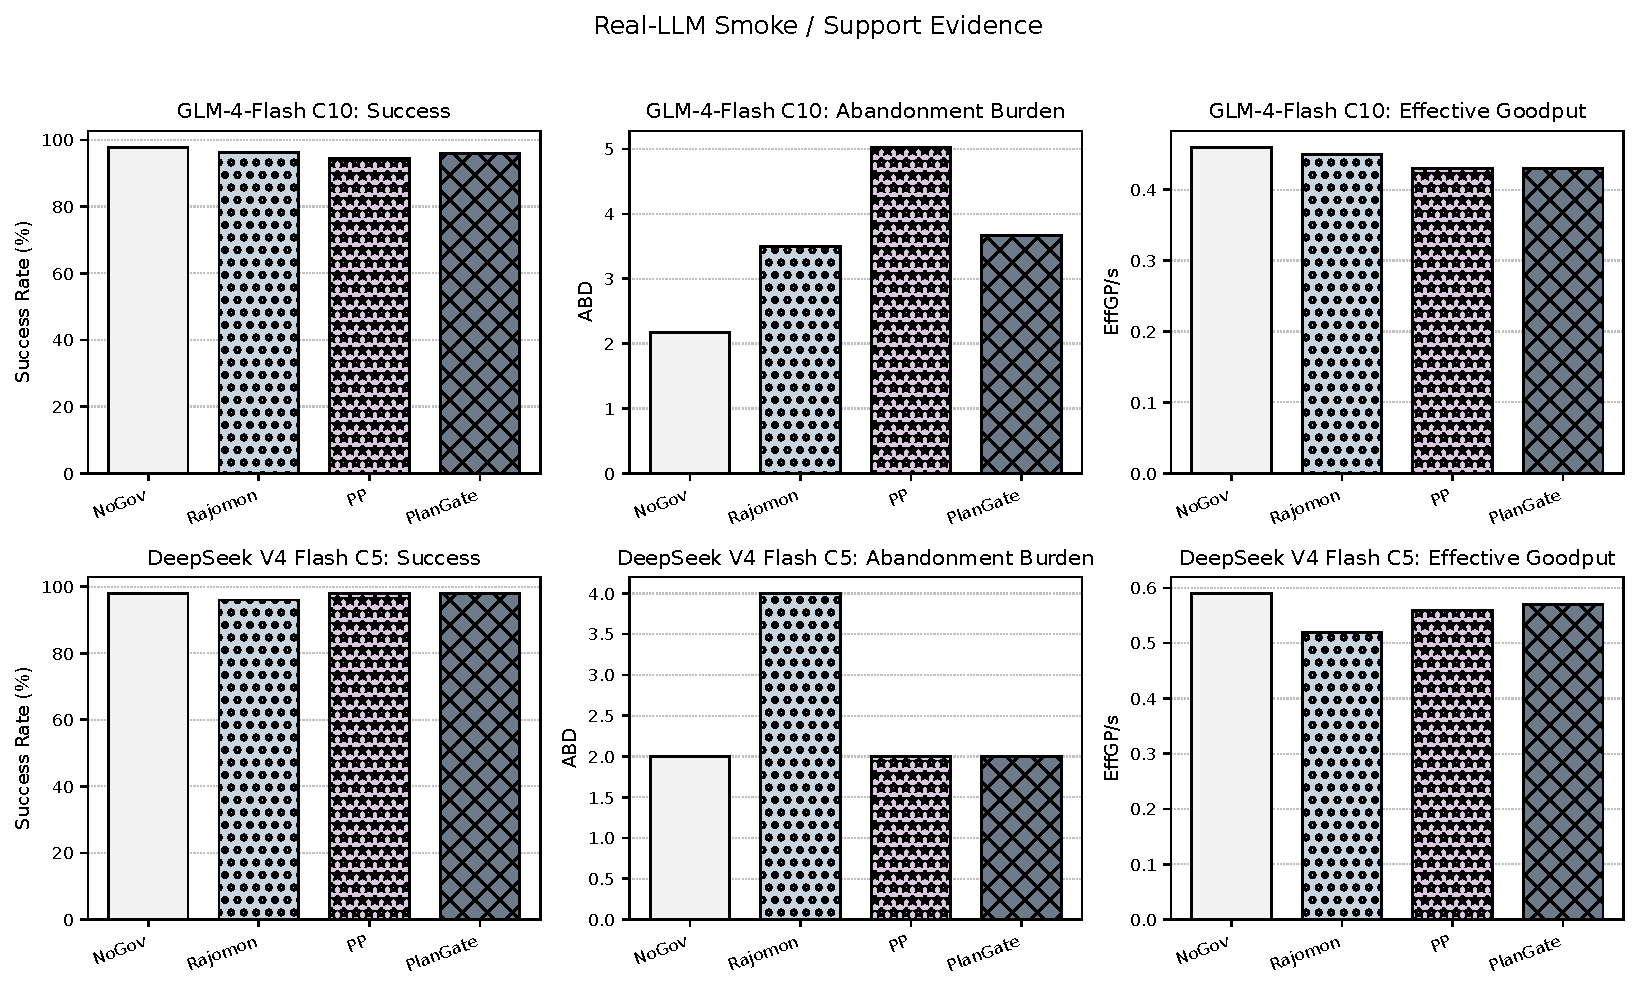
\includegraphics[width=\columnwidth]{fig_real_llm_smoke}
\caption{Provider-backed smoke evidence from GLM and DeepSeek runs. These runs are included as compatibility and boundary evidence: they confirm that the ReAct client, tool-call handling, and gateway policies operate against real provider APIs, while provider elasticity and model-specific behavior prevent a universal ``PlanGate wins all'' interpretation.}
\label{fig:real_llm_smoke}
\end{figure}

\textbf{Provider smoke evidence.}
The DeepSeek and GLM rows in Table~\ref{tab:reallm}, together with
Figure~\ref{fig:real_llm_smoke}, should be read as compatibility and boundary
evidence. They show that provider-side tool-call execution remains stable and
that PlanGate does not introduce obvious integration failures, but they are not
used as universal dominance evidence.


\subsection{Bursty Real-LLM: Waste Reduction Under Backend-Limited Burst Overload}
\label{sec:bursty_reallm}

The steady-state experiments (\S\ref{sec:reallm}) operate in a regime where provider-managed rate limits absorb most contention. To test session commitment under \emph{backend-capacity-limited} burst overload---where contention arises from finite tool-server workers rather than LLM provider throttling---we conduct a bursty real-LLM experiment using GLM-4-Flash with 10 backend workers and burst arrival at $C{=}20$ (30 sessions per burst, 8\,s inter-burst gap, \texttt{max\_steps=15}), measuring PARTIAL (wasted tool calls on doomed sessions), ABD, and cross-run variance as primary metrics. PlanGate is configured with \texttt{max\_sessions=12}, $\alpha{=}0.7$, \texttt{session\_cap\_wait=3}. We compare NG and PlanGate over $N{=}7$ repeats.

\textbf{Bottleneck characterization.}
Across all runs, zero HTTP~429 responses are observed from the LLM provider---confirming that the bottleneck lies entirely in backend tool-server capacity (10 workers), not provider-side rate limiting. This distinction is critical: the experiment tests session commitment under \emph{infrastructure scarcity} (finite workers) rather than API quota scarcity.

\begin{table}[t]
\caption{Bursty real-LLM validation ($N{=}7$, mean$\pm$std). Burst arrival: 30 sessions per burst, $C{=}20$, 10 backend workers. PARTIAL = doomed sessions (sessions that begin execution but ultimately fail).}
\label{tab:bursty_reallm}
\small
\resizebox{\columnwidth}{!}{%
\begin{tabular}{@{}lrrrrr@{}}
\toprule
\textbf{Gateway} & \textbf{PARTIAL$\downarrow$} & \textbf{Rej\textsubscript{0}} & \textbf{ABD\%} & \textbf{Succ.\%} & \textbf{Cascade$\downarrow$} \\
\midrule
NG        & $94\pm14$  & $86\pm15$ & $82.5\pm3.5$ & $10.0\pm2.4$ & $174\pm38$ \\
\textbf{PlanGate} & $\mathbf{76\pm12}$ & $108\pm12$ & $82.4\pm5.7$ & $8.1\pm2.8$ & $\mathbf{143\pm25}$ \\
\midrule
\multicolumn{6}{@{}l}{\footnotesize\textit{Two-sample $t$-test (df=12, pooled):}} \\
\multicolumn{6}{@{}l}{\footnotesize PARTIAL: $t{=}2.73$, $p{<}0.02$ ~~ Rej\textsubscript{0}: $t{=}3.13$, $p{<}0.01$} \\
\multicolumn{6}{@{}l}{\footnotesize Cascade: $t{=}1.84$ (one-tailed), $p{<}0.05$ ~~ ABD: n.s.} \\
\bottomrule
\end{tabular}}
\end{table}

Table~\ref{tab:bursty_reallm} presents three key findings:

\noindent\textbf{(1) Significant doomed-session reduction.}
PlanGate reduces doomed sessions (PARTIAL) from $94\pm14$ to $76\pm12$---a 19\% reduction that is statistically significant ($t(12){=}2.73$, $p{<}0.02$). The mechanism is explicit: PlanGate's sunk-cost pricing and session-cap mechanisms convert mid-session failures into zero-compute-waste step-0 rejections. Accordingly, PlanGate issues significantly more step-0 rejections ($108\pm12$ vs.\ $86\pm15$, $t(12){=}3.13$, $p{<}0.01$)---blocking sessions early rather than admitting them to fail after consuming resources.

\noindent\textbf{(2) ABD comparable; success rates similar.}
Both gateways exhibit similar ABD (NG: $82.5\pm3.5$\%, PG: $82.4\pm5.7$\%; n.s.) and success rates (NG: $10.0\pm2.4$\%, PG: $8.1\pm2.8$\%). PlanGate's numerically lower overall success percentage reflects its higher step-0 rejection count ($108$ vs.\ $86$): more sessions are blocked before execution, so fewer sessions enter the backend and have a chance to complete. The absolute success difference (PG: $16.1\pm5.6$ vs.\ NG: $20.0\pm4.8$ tasks per run) is not statistically significant ($t(12){=}1.39$, n.s.), though numerically PlanGate accepts fewer sessions. Under backend-limited burst overload, session commitment reduces the \emph{total number of doomed sessions} more clearly than it reduces the \emph{fraction} of admitted ones, because the backend worker bottleneck (10 workers) constrains total throughput equally across gateways.

\noindent\textbf{(3) Significant cascade waste reduction.}
Total wasted tool calls (Cascade) decrease from $174\pm38$ to $143\pm25$ ($-18.0$\%, $t(12){=}1.84$, one-tailed $p{<}0.05$)---approximately 31 fewer wasted steps per run. With $N{=}7$ repeats, the cascade reduction reaches one-tailed statistical significance, confirming that PlanGate's early rejection mechanism prevents not only shallow failures but also reduces cumulative wasted compute across the session population.

\textbf{Scope of claims.}
Under bursty real-LLM workloads, session commitment significantly reduces doomed sessions by converting mid-session failures to step-0 rejections---distinct from the provider-backed boundary/smoke setting in \S\ref{sec:reallm} and from the mock bursty robustness setting (ABD$\,{=}\,$0.4\%). Reducing $\sim$18 doomed sessions per run saves $\sim$31 cascade waste steps of LLM and backend compute. The comparable ABD under backend-limited burst reflects that PlanGate's primary benefit in this regime is \emph{waste reduction through early rejection} rather than success-rate improvement---a distinction that aligns with session commitment's goal of honoring admission decisions, not circumventing hard capacity constraints.

\textbf{Token waste quantification.}
As a separate token-efficiency diagnostic retained from earlier provider-backed traces, Figure~\ref{fig:token_efficiency} shows that PlanGate reduces agent LLM tokens per successful task by approximately 10\% under GLM-4-Flash (6{,}718\,$\to$\,6{,}049 tokens). Under DeepSeek-V3 the reduction is modest at $\sim$1.5\% (8{,}527\,$\to$\,8{,}401 tokens), reflecting that under that tokenization profile per-step counts leave less margin for commitment-driven savings. This token/fairness diagnostic figure is not from the same evidence bundle as the current boundary table built from \texttt{glm\_real\_llm\_c10\_refresh\_v1} and \texttt{deepseek\_v4\_flash\_smoke\_v1}; in particular, the DeepSeek-V3 token diagnostic should not be read as the DeepSeek-V4-Flash smoke run.

\begin{figure*}[t]
\centering
\begin{subfigure}[t]{0.48\textwidth}
\centering
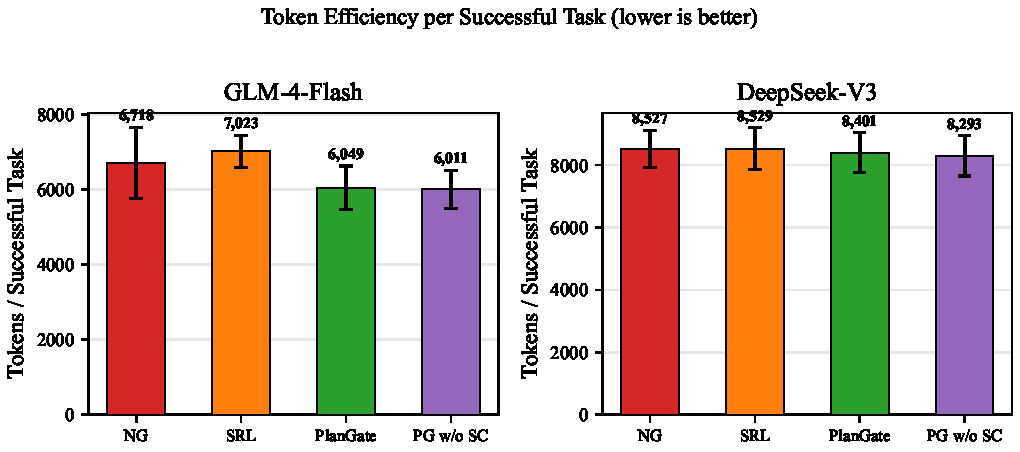
\includegraphics[width=\textwidth]{chart4_token_efficiency}
\caption{Agent LLM tokens per successful task.}
\label{fig:token_efficiency}
\end{subfigure}
\hfill
\begin{subfigure}[t]{0.48\textwidth}
\centering
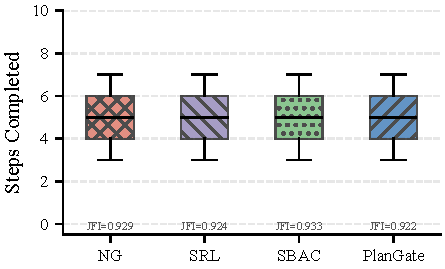
\includegraphics[width=\textwidth]{chart6_fairness}
\caption{Agent step distribution (boxplot).}
\label{fig:fairness}
\end{subfigure}
\caption{Efficiency and fairness diagnostics retained from earlier provider-backed traces. (a)~Figure~\ref{fig:token_efficiency} is a token-efficiency diagnostic: PlanGate achieves $\sim$10\% lower per-task token cost under GLM-4-Flash ($\sim$1.5\% under DeepSeek-V3), with savings driven by early commitment cutting cascade waste. (b)~Figure~\ref{fig:fairness} is a fairness diagnostic: step distribution and JFI remain comparable across gateways, showing that efficiency gains do not come from extreme step-level unfairness. These diagnostics are not the same evidence bundle as the current GLM C10 / DeepSeek C5 boundary table.}
\label{fig:efficiency_fairness}
\end{figure*}

\subsection{Self-Hosted vLLM: High-Contention Validation}
\label{sec:selfhosted}

To verify that PlanGate's governance operates correctly under self-hosted GPU inference---where the bottleneck is local compute rather than external API quotas---we conduct a supplementary experiment using Qwen-3.5-4B served via vLLM (\texttt{max-num-seqs=8}) as the backend LLM tool. The protocol is: $N{=}3$ repeats, 80 ReAct agents, $C{=}16$, burst arrival (12 per burst, 5\,s gap), \texttt{max\_steps=8}, and 8 backend/GPU workers, placing the system in a saturated backend-limited regime.

For the self-hosted vLLM stress setting, we report a \emph{backend-capacity-tuned} PlanGate configuration, denoted \emph{PlanGate (tuned)}, rather than the conservative admission profile used in earlier real-LLM smoke diagnostics. This is a display choice for this particular backend-limited regime, not a claim that the tuned configuration replaces the default PlanGate operating point in other experiments.

\begin{table}[t]
\caption{Self-hosted vLLM stress validation ($N{=}3$, Qwen-3.5-4B backend). 80 agents, $C{=}16$, 8 GPU workers. The submitted artifact contains the main-paper 5-gateway display subset.}
\label{tab:selfhosted}
\small
\resizebox{\columnwidth}{!}{%
\begin{tabular}{@{}lrrrrr@{}}
\toprule
\textbf{Gateway} & \textbf{Succ.\%} & \textbf{ABD\%} & \textbf{Rej} & \textbf{Cascade$\downarrow$} & \textbf{P95\,(s)} \\
\midrule
NG                & $\mathbf{24.2\pm14.4}$ & $\mathbf{72.1\pm15.5}$ & $11.7\pm3.2$ & $\mathbf{60.7\pm11.5}$ & $205.6\pm31.5$ \\
Static            & $16.2\pm5.0$          & $80.5\pm5.9$          & $13.3\pm0.6$ & $67.0\pm4.0$          & $204.6\pm43.4$ \\
PP                & $17.1\pm4.4$          & $78.5\pm4.3$          & $17.0\pm4.4$ & $66.3\pm3.5$          & $\mathbf{192.5\pm20.7}$ \\
Rajomon           & $21.7\pm3.1$          & $74.6\pm3.7$          & $11.7\pm2.9$ & $62.7\pm2.5$          & $204.4\pm35.4$ \\
PlanGate (tuned)  & $23.4\pm4.4$          & $74.2\pm4.2$          & $\mathbf{8.0\pm2.6}$  & $61.3\pm3.5$          & $222.7\pm54.3$ \\
\bottomrule
\end{tabular}}
\end{table}

\begin{figure}[t]
\centering
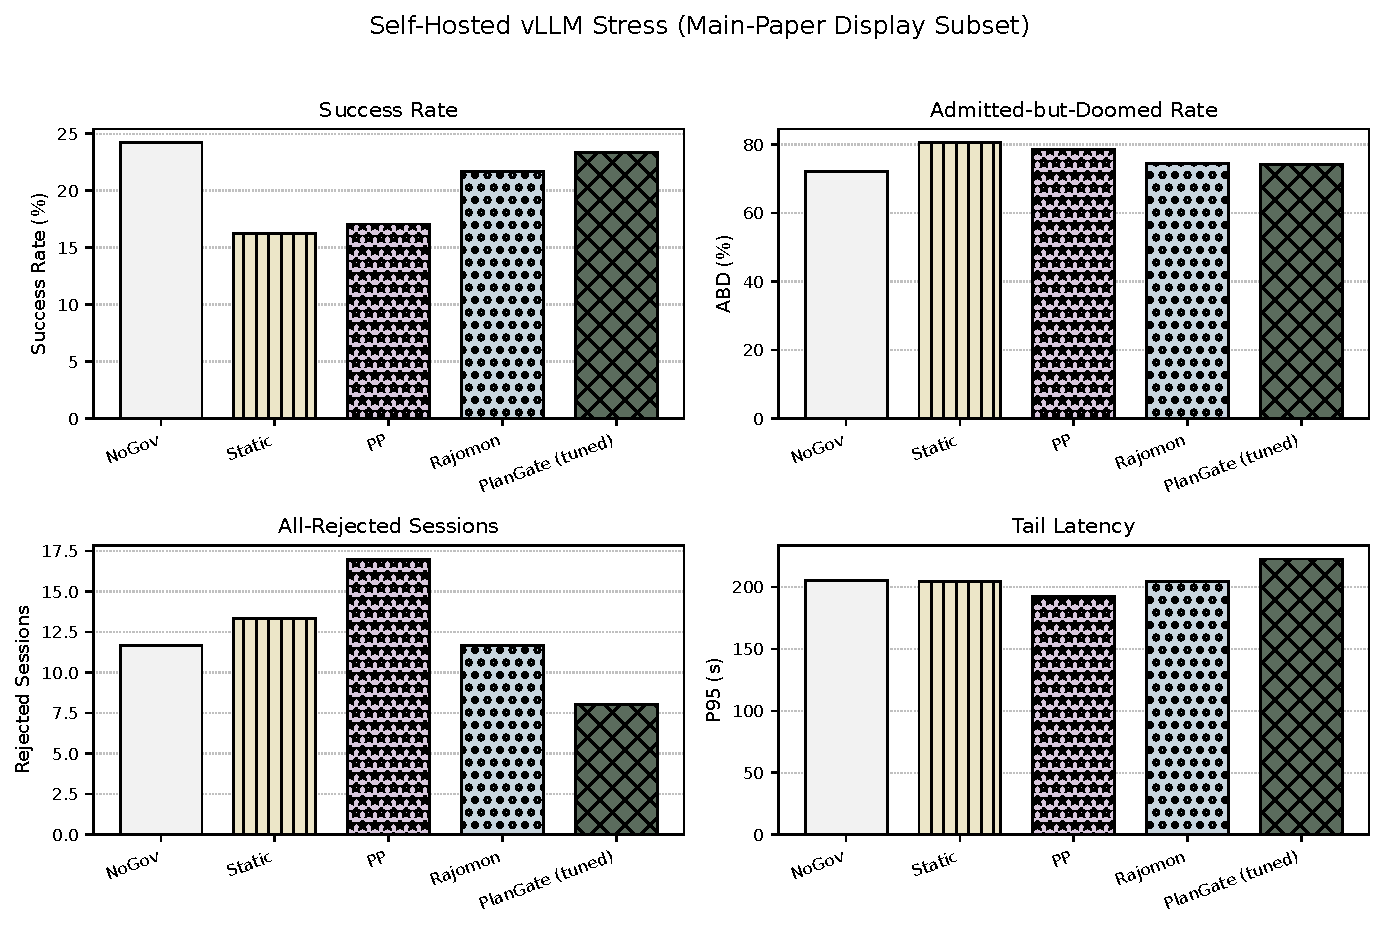
\includegraphics[width=\columnwidth]{fig_selfhosted_vllm_stress}
\caption{Self-hosted vLLM stress evidence from the main-paper display subset. The submitted artifact contains this 5-gateway subset and reports the backend-capacity-tuned PlanGate configuration for this saturated local-vLLM regime. A conservative diagnostic profile was used during local sensitivity checking but is not included in the submitted vLLM artifact.}
\label{fig:selfhosted_vllm}
\end{figure}

Under saturated GPU capacity, all gateways operate in a harsh regime: success remains low and ABD remains high because the backend itself is the hard bottleneck. The tuned PlanGate configuration is therefore best read as a \emph{boundary characterization} rather than a universal win: it restores PlanGate to the same qualitative band as NG and Rajomon on success and ABD, while achieving the lowest all-rejected count in the main-paper subset (8.0 vs.\ 11.7--17.0). The correct conclusion is not that governance creates capacity. Rather, the tuned configuration shows that once backend-local saturation is acknowledged explicitly, PlanGate can remain competitive on useful completion while avoiding the overly conservative admission profile seen in earlier diagnostics. Scaling GPU workers remains the primary remedy under full saturation; governance only shapes how scarce capacity is spent.

\subsection{Throughput--Latency Trade-off Under Increasing Concurrency}
\label{sec:tput_latency}

The mock and provider-backed sections above focus on mechanism and boundary
behavior. Here we summarize offered-load sweeps using
\texttt{artifact\_results/throughput\_latency\_summary\_v1}, which aggregates
existing Exp1/Exp5/Exp6/Exp10 CSV summaries rather than introducing a new
experiment. The sweep evidence is reported as effective goodput (sessions/s),
step-0 rejections, cascade failures, and P95 E2E latency of successful sessions.

\begin{figure*}[t]
\centering
\begin{subfigure}[t]{0.49\textwidth}
\centering
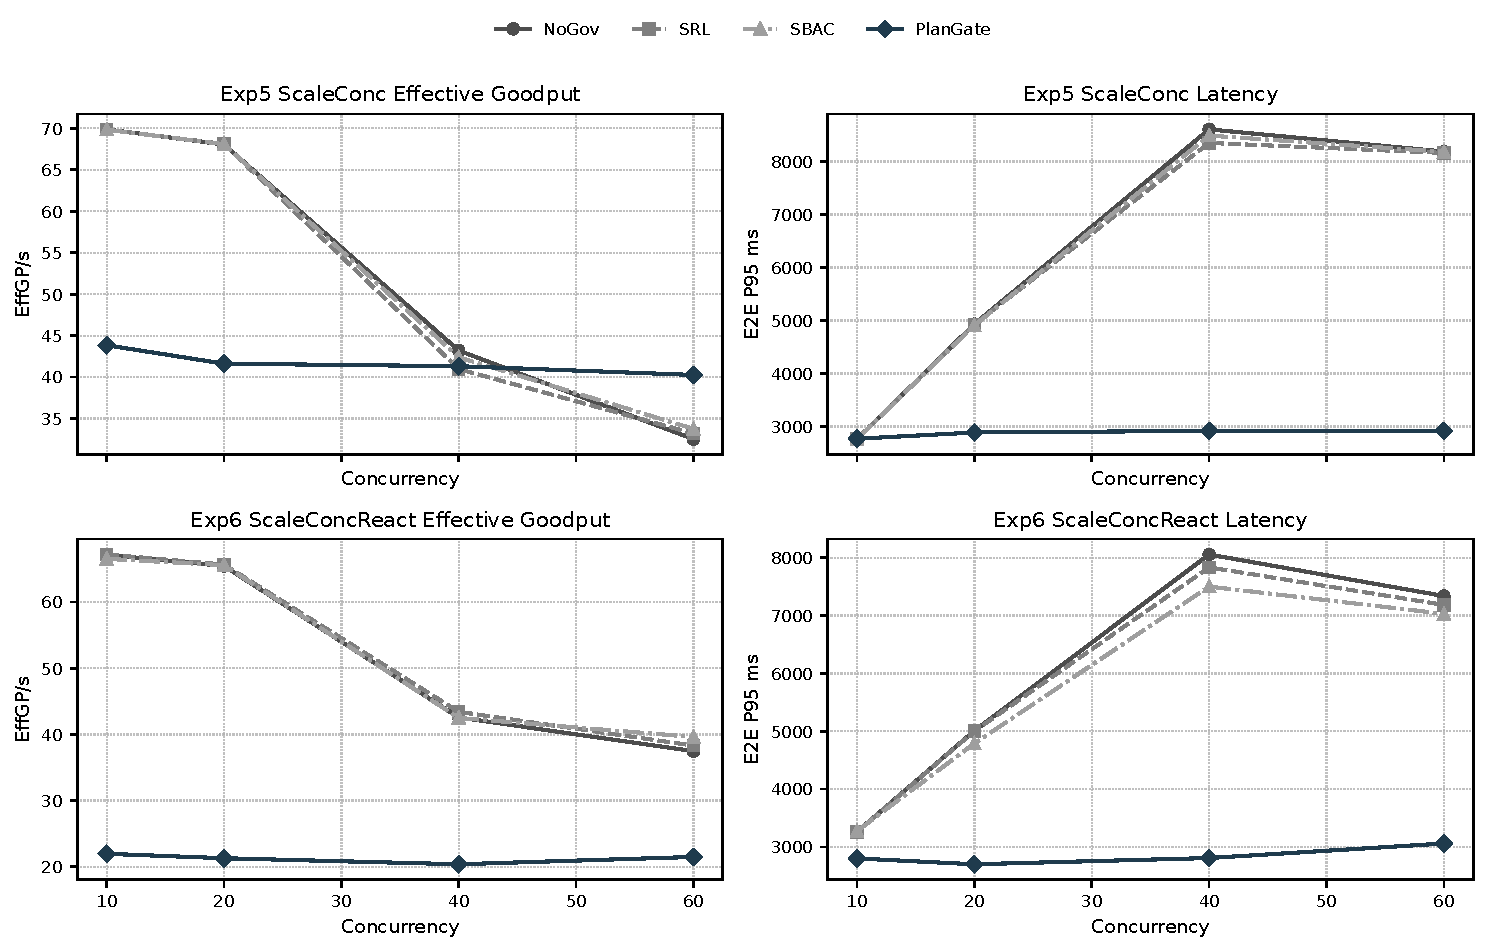
\includegraphics[width=\textwidth]{fig_scale_concurrency_effgp_latency}
\caption{Concurrency sweep: effective GP/s and P95.}
\label{fig:scale_conc_effgp_latency}
\end{subfigure}
\hfill
\begin{subfigure}[t]{0.49\textwidth}
\centering
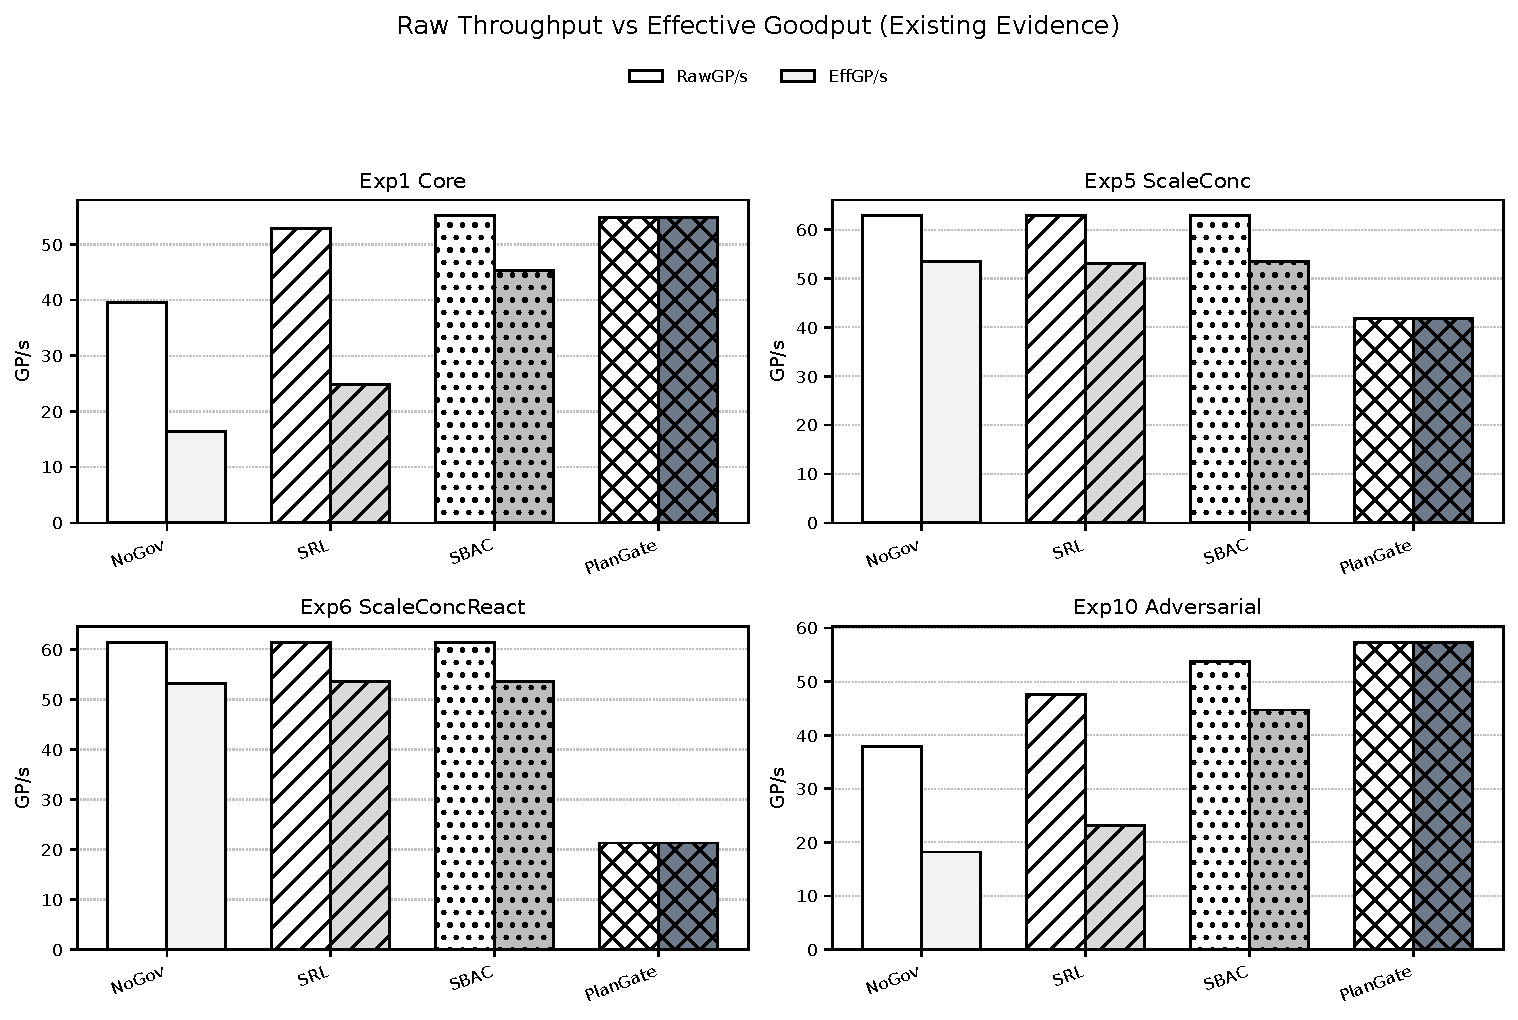
\includegraphics[width=\textwidth]{fig_throughput_effective_goodput}
\caption{Raw vs.\ effective goodput across existing summaries.}
\label{fig:throughput_effective_goodput}
\end{subfigure}
\caption{Throughput and latency evidence consolidated from Exp1/Exp5/Exp6/Exp10 artifact summaries. The left panel shows the overload transition; the right panel separates raw work admitted from effective work that contributes to completed sessions.}
\label{fig:tput_latency}
\end{figure*}

\textbf{Results (Table~\ref{tab:tput_latency}; Figure~\ref{fig:tput_latency}).}
Using representative Exp5 concurrency points from
\texttt{throughput\_latency\_summary\_v1}, three trends are clear.

\emph{Under-load ($C{=}10$).}
NG/SRL/SBAC are effectively identical (EffGP ${\approx}69.9$\,sess/s, P95
${\approx}2.76$\,s, zero cascades). PlanGate is more conservative (EffGP
43.8\,sess/s) with high step-0 rejection (138.6), reflecting admission overhead
when capacity is not yet tight.

\emph{Overload onset ($C{=}40$).}
NG/SRL/SBAC fall to 41--43\,sess/s with P95 around 8.35--8.61\,s and cascade
fractions 41.8--46.5\%. PlanGate keeps cascade at 0.0\% and lowers P95 to
2.92\,s while remaining in the same effective-goodput band (41.3\,sess/s).

\emph{Severe overload ($C{=}60$).}
PlanGate reaches the highest effective goodput (40.3\,sess/s) with the lowest
P95 (2.92\,s) and 0.0\% cascade, while NG/SRL/SBAC remain at 32.5--33.8\,sess/s
and P95 around 8.16--8.19\,s with cascade fractions near 59--60\%.

\textbf{Interpretation.}
The summary supports a stable tradeoff story: PlanGate pays a conservative
admission cost at low load, then dominates the latency/waste frontier once the
system is overloaded. The mechanism remains the same across points: converting
would-be mid-session failures into step-0 rejection reduces queue pollution and
preserves useful completion under contention.

\begin{table}[t]
\centering
\caption{Representative throughput--latency rows from
\texttt{artifact\_results/throughput\_latency\_summary\_v1}
(Exp5\_ScaleConc, $N{=}5$). Effective goodput (sess/s) and P95 E2E latency (s)
of successful sessions. Cascade\% is computed over admitted sessions as
$\mathrm{Cascade}/(\mathrm{Success}+\mathrm{Cascade})$.}
\label{tab:tput_latency}
\small
\resizebox{\columnwidth}{!}{%
\begin{tabular}{@{}llrrrr@{}}
\toprule
\textbf{Load} & \textbf{Gateway} & \textbf{GP/s} & \textbf{P95 (s)} & \textbf{Casc.\%} & \textbf{Rej\textsubscript{0}} \\
\midrule
\multirow{4}{*}{\shortstack[l]{$C{=}10$\\(under-load)}}
  & NG              & $69.88$ & $2.76$ & $0.0$ & $0.0$ \\
  & SRL             & $69.85$ & $2.77$ & $0.0$ & $0.0$ \\
  & SBAC            & $69.84$ & $2.76$ & $0.0$ & $0.0$ \\
  & PlanGate        & $43.84$ & $2.77$ & $0.0$ & $138.6$ \\
\midrule
\multirow{4}{*}{\shortstack[l]{$C{=}40$\\(overload)}}
  & NG              & $43.20$ & $8.61$ & $42.1$ & $29.0$ \\
  & SRL             & $40.97$ & $8.35$ & $46.5$ & $29.6$ \\
  & SBAC            & $42.39$ & $8.49$ & $41.8$ & $30.8$ \\
  & PlanGate        & $41.32$ & $\mathbf{2.92}$ & $0.0$ & $145.4$ \\
\midrule
\multirow{4}{*}{\shortstack[l]{$C{=}60$\\(severe)}}
  & NG              & $32.52$ & $8.19$ & $60.0$ & $61.4$ \\
  & SRL             & $33.20$ & $8.16$ & $59.9$ & $61.4$ \\
  & SBAC            & $33.76$ & $8.18$ & $59.2$ & $70.0$ \\
  & PlanGate        & $\mathbf{40.26}$ & $\mathbf{2.92}$ & $0.0$ & $145.2$ \\
\bottomrule
\end{tabular}}
\end{table}

\subsection{Multi-Gateway Shared-State Validation}
\label{sec:multigateway}

The preceding experiments run a single PlanGate gateway process.
To test whether P\&S session commitment depends on process-local memory, we run a controlled two-gateway deployment with per-step routing.
Each run uses $S{=}300$ P\&S sessions, 10 backend workers, \texttt{max\_sessions=30}, and $N{=}5$ repeats at $C\in\{20,40,60\}$.
We compare three modes: \emph{Single-GW} (one gateway with in-memory reservation state), \emph{2xGW-NoShare} (two gateways, independent in-memory state, random routing at each step), and \emph{2xGW+Redis} (two gateways, random routing, Redis-backed shared P\&S reservation state).
This experiment is P\&S-only: it validates cross-gateway reservation and locked-price continuation, not ReAct shared continuation or PlanGate-R recovery.

\begin{table}[t]
\centering
\caption{Multi-gateway P\&S shared-state validation ($S{=}300$, $N{=}5$ repeats).
StateMiss\% is the percentage of sessions that encounter a continuation state miss; it is the primary semantic-failure metric for this experiment.
Cross\% is the percentage of sessions whose steps execute on both gateway nodes.
MaxAct is the peak admitted-session count reconstructed from traces.}
\label{tab:multigateway}
\small
\resizebox{\columnwidth}{!}{%
\begin{tabular}{@{}llrrrrrrr@{}}
\toprule
\textbf{Mode} & \textbf{C} & \textbf{Succ\%} & \textbf{Rej0\%} & \textbf{StateMiss\%} & \textbf{Cross\%} & \textbf{MaxAct} & \textbf{GP/s} & \textbf{P95(ms)} \\
\midrule
\multirow{3}{*}{Single-GW}
  & 20 & 17.6 & 82.4 & 0.0 & 0.0 & 17 & 5.96 & 2941 \\
  & 40 & 20.1 & 79.9 & 0.0 & 0.0 & 20 & 5.85 & 3301 \\
  & 60 & 18.6 & 81.4 & 0.0 & 0.0 & 20 & 5.79 & 3214 \\
\midrule
\multirow{3}{*}{2xGW-NoShare}
  & 20 & 3.1 & 68.5 & 28.5 & 28.5 & 3 & 1.06 & 2292 \\
  & 40 & 4.8 & 66.1 & 29.1 & 29.1 & 4 & 1.53 & 2701 \\
  & 60 & 3.9 & 66.1 & 30.1 & 30.1 & 3 & 1.25 & 1884 \\
\midrule
\multirow{3}{*}{2xGW+Redis}
  & 20 & 26.1 & 73.8 & 0.0 & 22.8 & 20 & 6.52 & 4606 \\
  & 40 & 22.1 & 77.3 & 0.0 & 19.7 & 31 & 6.51 & 5334 \\
  & 60 & 22.0 & 77.3 & 0.0 & 20.1 & 31 & 6.10 & 5934 \\
\bottomrule
\end{tabular}}
\end{table}

Table~\ref{tab:multigateway} shows a clean semantic contrast.
Without shared state, random per-step routing causes continuation state misses for 28.5--30.1\% of sessions (427--451 state-miss events across five repeats per load point).
These misses track the cross-node session rate, indicating that the failure mode is not ordinary overload but loss of reservation context when a later step reaches a different gateway process.
With Redis-backed reservation state, state misses drop to zero while 19.7--22.8\% of sessions still cross gateway nodes.
The reconstructed active-session peak remains near the configured global cap (20--31), and Redis leak checks after the full run report \texttt{pg:active\_sessions=0} with no residual admission or reservation keys.

\textbf{CloudLab checkpoint-store validation.}
The newer CloudLab artifact repeats the same semantic question with the post-P3 checkpoint-store path enabled and random routing across gateways. Across 843 cross-node sessions, Redis-backed state records \texttt{state\_miss=0}, \texttt{duplicate\_admission=0}, and zero commitment invalid, mismatch, or expiry events. This does not make Redis a fault-tolerant control plane by itself, but it closes the main implementation gap in the earlier local validation: reservation, commitment, and checkpoint metadata can be looked up correctly when a session crosses gateway processes.

\textbf{Interpretation.}
Sticky routing, reported in the artifact but omitted from the main table, also eliminates state misses by keeping each session on one node.
However, stickiness is a routing-locality assumption rather than shared session governance: it avoids cross-node continuation rather than making continuation state available across nodes.
The Redis result supports the narrower deployment claim we need here: P\&S session commitment can be preserved beyond a single gateway process when reservation state is shared.
It does not evaluate shared ReAct progress, distributed reputation, or distributed price-state synchronization.

\subsection{Gateway Processing Overhead}
\label{sec:gateway_overhead}

We benchmark the governance path separately to distinguish control-plane cost from the throughput--latency gains attributed to session commitment. The focused Go microbenchmarks on this workstation place the core paths in the microsecond range: DAG validation grows from 1.74~$\mu$s/op at 5 steps to 10.42 and 24.06~$\mu$s/op at 10 and 20 steps, session lookup sits at about 0.33~$\mu$s/op for both budget reservations and ReAct state, P\&S first-step admission is 40.41~$\mu$s/op, and the HTTP \texttt{tools/call} ReAct path is 15.81~$\mu$s/op. Price computation is effectively free at 0.0004~$\mu$s/op (sub-nanosecond). These costs are far below the latency of mock heavy tools and real LLM service time, so the main benefit of PlanGate cannot be explained by a faster request path.

\begin{table}[t]
\centering
\caption{Gateway processing overhead on this workstation (focused Go microbenchmarks; mean per operation). The purpose is to bound governance cost, not to claim the request path is faster than a no-governance baseline.}
\label{tab:gateway_overhead}
\small
\resizebox{\columnwidth}{!}{%
\begin{tabular}{@{}lrrl@{}}
\toprule
\textbf{Path} & \textbf{Time ($\mu$s/op)} & \textbf{Allocs/op} & \textbf{Interpretation} \\
\midrule
DAG validation (5-step) & 1.74 & 7 & plan parsing and topological checks are negligible \\
P\&S first-step admission (5-step) & 40.41 & 63 & admission remains small relative to tool execution \\
ReAct \texttt{tools/call} ServeHTTP & 15.81 & 32 & request routing stays in the low-microsecond regime \\
\bottomrule
\end{tabular}%
}
\end{table}

The live trace collection in the appendix is retained as a diagnostic signal only: it records gateway-observed service time from \texttt{gateway\_latency\_us}, which may include proxied backend/tool execution and is therefore not treated as pure gateway processing overhead evidence. Accordingly, the main overhead claim in this section is grounded in the focused Go microbenchmarks above; the conservative interpretation remains unchanged: gains in overloaded regimes come from reducing doomed sessions and queue pollution, not from a shorter per-request control path.

\subsection{Reliability Checks}
\label{sec:fairness}
\label{sec:stats}

Fairness checks, computed separately from step-level execution traces, show comparable Jain Fairness Index across all gateways in the core mock comparison, reflecting binary admission rather than mid-session interruption. The statistical pattern matches the evidence hierarchy: mock and controlled failure-specific signals remain the primary causal evidence; provider-backed GLM/DeepSeek runs are interpreted as compatibility and boundary evidence rather than formal significance surfaces; bursty results remain significant for PARTIAL ($p{<}0.02$) and Rej\textsubscript{0} ($p{<}0.01$), with cascade waste reduction at one-tailed $p{<}0.05$. The new failure/amendment ablation is validated by deterministic mechanism signals (for example, zero amendment success when amendment is disabled and zero recovery success when recovery is disabled) rather than by treating effective goodput alone as the success criterion.

\subsection{Controlled Runtime Recovery Evaluation}
\label{sec:recovery-eval}

We evaluate PlanGate-R (\S\ref{sec:recovery-ext}) in a controlled mock runtime that exercises the actual \texttt{MCPDPServer} HTTP routing path, including automatic checkpoint creation after successful steps, recovery-eligible marking after classified recoverable failures, and the full \texttt{X-Recovery-Mode} resume path.
Mock tool handlers inject natural handler-level recoverable failures; no real LLM is used.
The experiment is P\&S mode only and is not a production benchmark.

\textbf{Setup.}
Each run submits $S{=}50$ P\&S sessions with $N{=}5$ declared steps.
Recoverable failures are injected at step~2 via Bernoulli sampling with failure rate $r{=}0.3$ (sensitivity across $r\in\{0.1,0.3,0.5\}$ appears in Supplementary Material, Section~7).
Five independent seeds provide variance estimates.
Three policies are compared:
\emph{PlanGate-base} (no recovery, failed sessions terminate),
\emph{naive retry} (full session restart from step~0), and
\emph{PlanGate-R} (checkpoint-based resume from the last completed step).

\textbf{Results.}
Table~\ref{tab:plangate_r_recovery} presents the main results.
PlanGate-base achieves $0.704\pm0.055$ success rate, terminating sessions on failure without a recovery path and leaving approximately 14.8~sessions per run abandoned after partial progress.
Naive retry achieves $1.000\pm0.000$ success by restarting from scratch, but at the cost of $294.4\pm8.3$ total tool calls per run and $44.4\pm8.3$ waste steps.
In this controlled mock runtime under injected recoverable failures, PlanGate-R matches naive retry in eventual completion ($1.000\pm0.000$) while reducing tool calls to $264.8\pm2.8$ per run---a saving of $29.6$~calls attributable to avoided prefix replay---and reducing waste steps from $44.4$ to $14.8\pm2.8$ ($-66.7\%$).
Calls-per-successful-session decrease from $5.89$ (naive) to $5.30$ (PlanGate-R).
Avoided replay scales with failure rate: $8.8$~calls/run at $r{=}0.1$; $52.4$ at $r{=}0.5$.

\textbf{Interpretation.}
The benefit of PlanGate-R is lower replay waste at comparable eventual completion, not a universal reduction in failure probability.
Under failure modes not classified as recoverable, PlanGate-R degrades gracefully to the same behavior as PlanGate-base: the session terminates rather than resuming unsoundly.
These results are scoped to the controlled mock runtime described above and should not be extrapolated to real-LLM workloads or arbitrary failure distributions. Distributed lookup of checkpoint/reservation metadata is validated separately in \S\ref{sec:multigateway}; replicated-store failure tolerance is not evaluated.

\textbf{Connection to the mechanism ablation.}
The failure/amendment ablation in Table~\ref{tab:p3_failure_mech} exercises the same recovery path under a larger workload with commitment and amendment toggles. Its signal is qualitative rather than a replacement for the controlled replay-waste table: disabling recovery drives recovery success to zero and increases cascade failures from 7.7 to 42.0, while disabling amendment drives amendment success to zero. Together, the two experiments show that checkpoint recovery reduces prefix replay when the failure is recoverable, and that the commitment/amendment guards are the mechanisms that keep recovery-scoped plan changes bounded.

\begin{table}[t]
\centering
\caption{Controlled runtime recovery evaluation under injected recoverable failures
  (\textit{failure\_rate}$\,{=}\,0.3$, $S{=}50$ sessions, $N{=}5$ steps, failure injected at step~2,
  5 independent seeds; P\&S mode only; mock handlers, no real LLM).
  \emph{Recovered} = sessions rescued via checkpoint resume per run.
  \emph{Waste Steps} = tool-call steps that do not contribute to the final successful trajectory,
  including discarded prefix work and failed interrupted calls.
  \emph{Avoided Replay} = steps saved by PlanGate-R relative to naive retry (mean over seeds).}
\label{tab:plangate_r_recovery}
\small
\resizebox{\columnwidth}{!}{%
\begin{tabular}{@{}lrrrrrr@{}}
\toprule
\textbf{Policy}     & \textbf{Success Rate}    & \textbf{Recovered} & \textbf{Tool Calls}    & \textbf{Waste Steps}  & \textbf{Calls/Succ.}   & \textbf{Avoided Replay} \\
\midrule
PlanGate-base       & $0.704\pm0.055$          & $0.0$              & $220.4\pm5.5$          & $44.4\pm8.3$          & $6.28\pm0.35$          & $0.0$                   \\
Naive retry         & $1.000\pm0.000$          & $0.0$              & $294.4\pm8.3$          & $44.4\pm8.3$          & $5.89\pm0.17$          & $0.0$                   \\
\textbf{PlanGate-R} & $1.000\pm0.000$          & $14.8$             & $\mathbf{264.8\pm2.8}$ & $\mathbf{14.8\pm2.8}$ & $\mathbf{5.30\pm0.06}$ & $\mathbf{29.6}$         \\
\bottomrule
\end{tabular}}
\vspace{-0.3em}
{\footnotesize \textit{Controlled mock runtime only; results do not transfer to real-LLM workloads or arbitrary failure distributions; not a ReAct semantic recovery experiment.}}
\end{table}


\section{Related Work}

\textbf{LLM agents and tool protocols.} ReAct~\cite{react} and Plan-and-Solve~\cite{planandsolve} expose different admission information: ReAct reveals only the next action, whereas P\&S-style agents can expose an upfront tool-call plan. MCP~\cite{mcp2024} standardizes tool invocation, but does not specify session-level overload semantics. PlanGate targets this missing governance layer.

\textbf{Tool-using and multi-agent LLM systems.} Tool-using and agent frameworks such as Toolformer~\cite{toolformer}, Chameleon~\cite{chameleon}, Gorilla~\cite{gorilla}, API-Bank~\cite{apibank}, LangChain~\cite{langchain}, CrewAI~\cite{crewai}, AutoGen~\cite{autogen}, Voyager~\cite{voyager}, Tree of Thoughts~\cite{tot}, and Graph of Thoughts~\cite{got} expand the range of workloads in which LLMs plan, call tools, coordinate agents, or execute multi-step tasks. These systems motivate PlanGate's workload model: they create dependent action sequences whose intermediate results are valuable only if the overall task completes. They generally leave overload governance to the underlying API gateway, serving stack, or application code; PlanGate instead provides a gateway-level mechanism for admitting and protecting such multi-step sessions.

\textbf{LLM serving systems.} Systems such as vLLM/PagedAttention~\cite{vllm}, Orca~\cite{orca}, SARATHI~\cite{sarathi}, Parrot~\cite{parrot}, DistServe~\cite{distserve}, FlexGen~\cite{flexgen}, and $S^3$~\cite{s3} improve LLM serving throughput, latency, batching, memory management, or application-level scheduling. They operate primarily inside the model-serving substrate, whereas PlanGate governs the admission and continuation of multi-step tool sessions before requests reach the backend. The two directions are complementary: a PlanGate deployment can sit in front of an optimized LLM serving backend while preserving session-level semantics.

\textbf{Overload control and request pricing.} Static rate limiting and classic adaptive overload-control mechanisms~\cite{leaky_bucket,overload_survey} govern traffic at request or connection granularity. Microservice systems such as DAGOR~\cite{dagor}, Breakwater~\cite{breakwater}, and Rajomon~\cite{rajomon2025} control overload at request or RPC granularity. They do not distinguish a session's first request from its later requests, where sunk compute is larger. PlanGate instead aligns the governance unit with the multi-step session.

\textbf{API gateways and service governance.} Envoy~\cite{envoy} and Kong~\cite{kong} provide mature routing, filtering, and rate-limiting frameworks. Their native abstractions are request-level; approximating session commitment requires custom stateful extensions that maintain per-session plans, locked prices, and continuation pricing (Supplementary Material, Section~1). PlanGate contributes the session-level governance engine rather than a replacement for production transport frameworks. In our evaluation, SBAC and Rajomon+SB serve as empirical proxies for the strongest plausible gateway extensions: session-token admission and session-aware per-request pricing; the appendix-only Envoy/Kong-style approximation table in Supplementary Material, Section~1 records the corresponding request-local baselines at $C{=}40$.

\textbf{Scheduling, isolation, and fairness.} Datacenter schedulers such as Shenango~\cite{shenango} and Caladan~\cite{caladan} reduce interference for latency-sensitive workloads through fast resource allocation and isolation. They address CPU scheduling and datacenter interference rather than semantic admission for dependent tool-call sessions. PlanGate's fairness reporting uses Jain's fairness index~\cite{jain_fairness}, but its primary objective is different: minimizing admitted-but-doomed sessions and wasted continuation work under multi-step dependencies.

\section{Discussion, Limitations, and Threats to Validity}

\textbf{Discount design and adaptation.}
The $K^2$ discount is one instantiation of session commitment, not the core contribution. The model in \S\ref{sec:discount-rationale} motivates it by reducing expected waste from $O(N^2)$ to $O(\ln N)$ under simplified assumptions; the discount function ablation (\S\ref{sec:discountablation}) confirms that aggressive discounters (exponential and quadratic) reduce cascades more than linear or logarithmic alternatives. We choose $K^2$ over $e^K$ because it is cheap to compute and grows less permissive for very deep sessions. Future work could adapt $\alpha$ online: increase it when ABD exceeds a target, and decrease it when step-0 rejections exceed a utilization target. Our $\alpha$ sweep suggests a wide operating envelope rather than a brittle hyperparameter. The load-modulation coefficient $\beta$ is similarly not a brittle constant: the Supplementary Material, Section~3 sweep over $\beta\in\{0,0.5,1,2,3\}$ shows identical completion counts across all settings, with only small cascade/fairness tradeoffs.

\textbf{Checkpointing and recovery.}
PlanGate-R (\S\ref{sec:recovery-ext}, \S\ref{sec:recovery-eval}) complements, rather than replaces, PlanGate's admission integrity: base session commitment prevents governance-induced mid-session failures, while PlanGate-R handles the orthogonal case of recoverable transient backend interruptions within already-admitted P\&S sessions.
In the controlled mock runtime, PlanGate-R achieves eventual success comparable to naive retry under injected recoverable failures while reducing replay waste by $66.7\%$ and tool calls by $10.1\%$ per run; whether this holds under real-world backend behavior with heterogeneous failure modes has not been evaluated, and we do not claim it transfers directly.
Five limitations govern this result.
\emph{First}, PlanGate-R is P\&S-only: ReAct sessions expose no pre-declared DAG against which to verify prefix soundness; ReAct semantic recovery would require client-cooperative observation traces and is not implemented.
\emph{Second}, checkpoint durability is store-dependent: the local mechanism tests use in-memory checkpoints, while CloudLab uses Redis to validate cross-node lookup; replicated-store failure tolerance remains outside this evaluation.
\emph{Third}, the resume path re-executes the declared DAG without semantic re-planning, and is suitable only when the original plan remains valid after the interruption.
\emph{Fourth}, the prototype includes quota logic for bounding recovery concurrency, but this controlled runtime experiment does not evaluate full multi-tenant scheduling between recovery and fresh sessions, which remains future work.
\emph{Fifth}, the resume path introduces non-trivial routing overhead that is not quantified in this evaluation.
Checkpoint-aware recovery is a natural complement to session commitment; the current evaluation is bounded to controlled P\&S workloads and should be read alongside the failure/amendment mechanism ablation rather than as a production recovery benchmark.

\textbf{Generalization and deployment.}
The main experiments evaluate a 10-tool ecosystem spanning light and heavy costs. More tools would extend the weight table, but production deployments may require finer-grained weights, tool-specific quotas, and multi-node shared state for reservations, prices, checkpoints, and reputation. Section~\ref{sec:multigateway} validates a first step beyond process-local state: for P\&S sessions, Redis-backed shared state preserves continuation semantics under random two-gateway routing and CloudLab records zero state misses across 843 cross-node sessions. This does not make the prototype a complete distributed control plane. Shared ReAct progress, distributed reputation, dynamic price-state synchronization, node-failure recovery, and production-grade store replication remain future work. Mock workloads use \texttt{time.sleep} to isolate admission behavior; real-LLM steady, bursty, self-hosted, GLM, and DeepSeek smoke experiments mitigate this realism threat but do not replace production traces.

\textbf{Real-provider interpretation.}
Provider-backed experiments are intentionally interpreted conservatively. Commercial APIs add hidden queuing, elastic rate-limit headroom, stochastic generation latency, and provider-specific tool-call response behavior. The GLM and DeepSeek evidence is therefore used as smoke/support and boundary characterization rather than as headline dominance evidence. The core causal claims remain grounded in controlled workloads where backend capacity and failure injection are known.

\textbf{Availability.}
The anonymized artifact contains the Go gateway, Python backend, agent clients, evaluation scripts, figure-generation scripts, and reproduction instructions for the no-key controlled mock experiments on a single machine. Provider-backed real-LLM experiments require API credentials and provider availability for live reruns. Lightweight evidence packages under \texttt{artifact\_results/} record the exact CSV summaries, validation checks, and SHA256 hashes used for the figures in \texttt{paper/figures}.

\section{Conclusion}

We presented \emph{session commitment}---the conjunction of atomic admission, temporal isolation, and continuation value---as a governance abstraction for multi-step LLM agent workloads, and implemented it in PlanGate, a plan-aware MCP-compatible gateway. Budget-reserved commitments for P\&S agents provide scoped price-isolation protection within declared plans; soft commitments for ReAct agents provide sunk-cost-aware continuation incentives---these are intentionally different guarantees, reflecting the fundamental information asymmetry between the two agent types. The updated implementation adds commitment tokens, bounded recovery-only amendment, checkpoint-aware recovery, and Redis-backed shared state. Our evaluation delineates session commitment's benefit boundary:
\emph{(i)}~Under hard capacity limits (mock), PlanGate reduces price-induced cascade failures to near-zero under controlled assumptions and delivers $3.4\times$ effective goodput over no-governance baselines.
\emph{(ii)}~Under provider-backed boundary/smoke evidence (GLM C10 refresh and DeepSeek C5), all gateways complete cleanly with zero client/runtime errors; PlanGate remains in a competitive band but does not claim universal dominance, so this layer is used as compatibility/boundary evidence rather than headline significance.
\emph{(iii)}~Under bursty real-LLM workloads with backend-capacity bottlenecks ($N{=}7$), PlanGate significantly reduces doomed sessions by ${\sim}19$\% ($p{<}0.02$) and cascade waste by ${\sim}18$\% (one-tailed $p{<}0.05$) by converting mid-session failures into zero-compute-waste step-0 rejections.
\emph{(iv)}~Under failure/amendment workloads, disabling commitment, amendment, or recovery removes the corresponding semantic signal and degrades session completion; disabling recovery increases cascade failures from 7.7 to 42.0.
In controlled two-gateway and CloudLab validations, Redis-backed state eliminates continuation state misses under random cross-node routing, including 843 cross-node CloudLab sessions with zero state misses. Session commitment's value scales with resource-constraint severity: large gains under hard limits, waste reduction under bursty overload, and a provider-backed boundary regime where compatibility remains stable but dominance is not universal. PlanGate operates as a transparent reverse proxy requiring only lightweight header annotations, providing a principled foundation for session-aware governance as LLM agent deployments scale.



% REFERENCES
\begin{thebibliography}{99}

\bibitem{react}
S. Yao, J. Zhao, D. Yu, N. Du, I. Shafran, K. Narasimhan, and Y. Cao.
\newblock ReAct: Synergizing Reasoning and Acting in Language Models.
\newblock In \emph{ICLR}, 2023.

\bibitem{planandsolve}
L. Wang, W. Xu, Y. Lan, Z. Hu, Y. Lan, R. K.-W. Lee, and E.-P. Lim.
\newblock Plan-and-Solve Prompting: Improving Zero-Shot Chain-of-Thought Reasoning by Large Language Models.
\newblock In \emph{ACL}, 2023.

\bibitem{dagor}
H. Zhou, M. Chen, Q. Lin, J. Lv, S. He, D. Pei, and D. Zhang.
\newblock Overload Control for Scaling WeChat Microservices.
\newblock In \emph{ACM SoCC}, 2018.

\bibitem{breakwater}
I. Cho, A. Saeed, J. Fried, S. J. Park, M. Alizadeh, and A. Belay.
\newblock Overload Control for $\mu$s-scale RPCs with Breakwater.
\newblock In \emph{USENIX OSDI}, 2020.

\bibitem{rajomon2025}
J. Xing, A. Giannoukos, P. Loh, S. Wang, J. Qiu, H. M. Demoulin, K. Kallas, and B. C. Lee.
\newblock Rajomon: Decentralized and Coordinated Overload Control for Latency-Sensitive Microservices.
\newblock In \emph{USENIX NSDI}, 2025.
\bibitem{vllm}
W. Kwon, Z. Li, S. Zhuang, Y. Sheng, L. Zheng, C. H. Yu, J. Gonzalez, H. Zhang, and I. Stoica.
\newblock Efficient Memory Management for Large Language Model Serving with PagedAttention.
\newblock In \emph{ACM SOSP}, 2023.

\bibitem{orca}
G. Yu, J. S. Jeong, G.-I. Kim, S. Kim, and B.-G. Chun.
\newblock Orca: A Distributed Serving System for Transformer-Based Generative Models.
\newblock In \emph{USENIX OSDI}, 2022.

\bibitem{sarathi}
A. Agrawal, A. Panwar, J. Mohan, N. Kwatra, B. S. Gulavani, and R. Ramjee.
\newblock SARATHI: Efficient LLM Inference by Piggybacking Decodes with Chunked Prefills.
\newblock \emph{arXiv:2308.16369}, 2023.

\bibitem{parrot}
C. Lin, Z. Han, C. Zhang, Y. Yang, F. Yang, C. Chen, and L. Qiu.
\newblock Parrot: Efficient Serving of LLM-based Applications with Semantic Variable.
\newblock In \emph{USENIX OSDI}, 2024.
\bibitem{mcp2024}
Anthropic.
\newblock Model Context Protocol Specification.
\newblock Technical Report, 2024.
\newblock \url{https://modelcontextprotocol.io/specification}.

\bibitem{langchain}
H. Chase.
\newblock LangChain: Building Applications with LLMs through Composability.
\newblock Software, v0.1, 2022.
\newblock \url{https://github.com/langchain-ai/langchain}.

\bibitem{autogen}
Q. Wu, G. Bansal, J. Zhang, Y. Wu, B. Li, E. Zhu, L. Jiang, X. Zhang, S. Zhang, A. H. Awadallah, R. W. White, D. Burger, and C. Wang.
\newblock AutoGen: Enabling Next-Gen LLM Applications via Multi-Agent Conversation Framework.
\newblock In \emph{COLM}, 2024.
\bibitem{shenango}
A. Ousterhout, J. Fried, J. Behrens, A. Belay, and H. Balakrishnan.
\newblock Shenango: Achieving High CPU Efficiency for Latency-sensitive Datacenter Workloads.
\newblock In \emph{USENIX NSDI}, 2019.

\bibitem{caladan}
J. Fried, Z. Ruan, A. Ousterhout, and A. Belay.
\newblock Caladan: Mitigating Interference at Microsecond Timescales.
\newblock In \emph{USENIX OSDI}, 2020.

\bibitem{toolformer}
T. Schick, J. Dwivedi-Yu, R. Dess\`{\i}, R. Raileanu, M. Lomeli, E. Hambro, L. Zettlemoyer, N. Cancedda, and T. Scialom.
\newblock Toolformer: Language Models Can Teach Themselves to Use Tools.
\newblock In \emph{NeurIPS}, 2023.
\bibitem{sunkcost_econ}
H. R. Arkes and C. Blumer.
\newblock The Psychology of Sunk Cost.
\newblock \emph{Organizational Behavior and Human Decision Processes}, 35(1):124--140, 1985.

\bibitem{crewai}
J. Moura.
\newblock CrewAI: Framework for Orchestrating Role-Playing Autonomous AI Agents.
\newblock Software, v0.28, 2024.
\newblock \url{https://github.com/crewAIInc/crewAI}.

\bibitem{tot}
S. Yao, D. Yu, J. Zhao, I. Shafran, T. Griffiths, Y. Cao, and K. Narasimhan.
\newblock Tree of Thoughts: Deliberate Problem Solving with Large Language Models.
\newblock In \emph{NeurIPS}, 2023.

\bibitem{got}
M. Besta, N. Blach, A. Kubicek, R. Gerstenberger, M. Podstawski, L. Gianinazzi, J. Gajda, T. Lehmann, H. Niewiadomski, P. Nyczyk, and T. Hoefler.
\newblock Graph of Thoughts: Solving Elaborate Problems with Large Language Models.
\newblock In \emph{AAAI}, 2024.

\bibitem{voyager}
G. Wang, Y. Xie, Y. Jiang, A. Mandlekar, C. Xiao, Y. Zhu, L. Fan, and A. Anandkumar.
\newblock Voyager: An Open-Ended Embodied Agent with Large Language Models.
\newblock \emph{Transactions on Machine Learning Research}, 2024.
\bibitem{s3}
Y. Jin, C.-F. Wu, D. Brooks, and G.-Y. Wei.
\newblock $S^3$: Increasing GPU Utilization during Generative Inference for Higher Throughput.
\newblock In \emph{NeurIPS}, 2023.
\bibitem{leaky_bucket}
A. S. Tanenbaum and D. J. Wetherall.
\newblock \emph{Computer Networks}.
\newblock Pearson, 5th edition, 2011.

\bibitem{cot}
J. Wei, X. Wang, D. Schuurmans, M. Bosma, B. Ichter, F. Xia, E. Chi, Q. Le, and D. Zhou.
\newblock Chain-of-Thought Prompting Elicits Reasoning in Large Language Models.
\newblock In \emph{NeurIPS}, 2022.

\bibitem{llmsurvey}
W. X. Zhao, K. Zhou, J. Li, T. Tang, X. Wang, Y. Hou, Y. Min, B. Zhang, J. Zhang, Z. Dong, Y. Du, C. Yang, Y. Chen, Z. Chen, J. Jiang, R. Ren, Y. Li, X. Tang, Z. Liu, P. Liu, J.-Y. Nie, and J.-R. Wen.
\newblock A Survey of Large Language Models.
\newblock \emph{arXiv:2303.18223}, 2023.

\bibitem{chameleon}
P. Lu, B. Peng, H. Cheng, M. Galley, K. W. Chang, Y. N. Wu, S.-C. Zhu, and J. Gao.
\newblock Chameleon: Plug-and-Play Compositional Reasoning with Large Language Models.
\newblock In \emph{NeurIPS}, 2023.

\bibitem{gorilla}
S. G. Patil, T. Zhang, X. Wang, and J. E. Gonzalez.
\newblock Gorilla: Large Language Model Connected with Massive APIs.
\newblock \emph{arXiv:2305.15334}, 2023.

\bibitem{apibank}
M. Li, Y. Zhao, B. Yu, F. Song, H. Li, H. Yu, Z. Li, F. Huang, and Y. Li.
\newblock API-Bank: A Comprehensive Benchmark for Tool-Augmented LLMs.
\newblock In \emph{EMNLP}, 2023.

\bibitem{overload_survey}
M. Welsh and D. Culler.
\newblock Adaptive Overload Control for Busy Internet Servers.
\newblock In \emph{USITS}, 2003.

\bibitem{distserve}
Y. Zhong, S. Liu, J. Chen, J. Hu, Y. Zhu, X. Liu, X. Jin, and H. Zhang.
\newblock DistServe: Disaggregating Prefill and Decoding for Goodput-optimized Large Language Model Serving.
\newblock In \emph{USENIX OSDI}, 2024.
\bibitem{flexgen}
Y. Sheng, L. Zheng, B. Yuan, Z. Li, M. Ryabinin, B. Chen, P. Liang, C. R\'{e}, I. Stoica, and C. Zhang.
\newblock FlexGen: High-Throughput Generative Inference of Large Language Models with a Single GPU.
\newblock In \emph{ICML}, 2023.

\bibitem{jain_fairness}
R. Jain, D. Chiu, and W. Hawe.
\newblock A Quantitative Measure of Fairness and Discrimination for Resource Allocation in Shared Computer Systems.
\newblock \emph{DEC Research Report TR-301}, 1984.

\bibitem{envoy}
M. Klein \emph{et al.}
\newblock Envoy Proxy: C++ L7 Proxy and Communication Bus.
\newblock Software, v1.31, 2024.
\newblock \url{https://www.envoyproxy.io/}.

\bibitem{kong}
Kong Inc.
\newblock Kong: The Cloud-Native API Gateway.
\newblock Software, v3.x, 2024.
\newblock \url{https://konghq.com/}.

\end{thebibliography}

\end{document}
